%% \documentclass[handout,t]{beamer} % HANDOUT
%% \documentclass[handout,notes=show,t]{beamer} % NOTES
\documentclass[t]{beamer} % SLIDES
\usepackage{etex}

\usetheme{StefanAntti}                % page themes: StefanPlain, StefanFAU, StefanOsna
%% \usepackage{beamer-font-lucida}  % commercial Lucida Math font package (recommended)
%% \usepackage{beamer-font-charter} % commercial Charter Match font package
%% \usepackage{beamer-font-arev}    % use Arev fonts from TexLive (combine with document option "smaller")
\usepackage{beamer-tools-stefan}    % standard packages, definitions and macros

%%%% uncomment the following macro libraries as needed
%% %%
%% support macros for graphics with the PGF packages
%%

%% \mmpaper[black]{0}{0}{8}{5}, \xypaper{0}{0}{8}{5}
%%   draw fine grid in pgf picture so that objects can easily be positioned
%%   \mmpaper draws cm/mm blocks, while \xypaper is based on (x,y) coordinates
\newcommand{\mmpaper}[5][black!40!white]{
  \begin{pgfscope}
    \color{#1}
    \pgfsetlinewidth{.2mm}
    \pgfgrid[step={\pgfpoint{1cm}{1cm}}]{\pgfpoint{#2cm}{#3cm}}{\pgfpoint{#4cm}{#5cm}}
    \pgfsetlinewidth{.1mm}
    \pgfgrid[step={\pgfpoint{1mm}{1mm}}]{\pgfpoint{#2cm}{#3cm}}{\pgfpoint{#4cm}{#5cm}}
  \end{pgfscope}
}
\newcommand{\xypaper}[5][black!40!white]{
  \begin{pgfscope}
    \color{#1}
    \pgfsetlinewidth{.2mm}
    \pgfgrid[step={\pgfxy(1,1)}]{\pgfxy(#2,#3)}{\pgfxy(#4,#5)}
    \pgfsetlinewidth{.1mm}
    \pgfgrid[step={\pgfxy(.1,.1)}]{\pgfxy(#2,#3)}{\pgfxy(#4,#5)}
  \end{pgfscope}
}

%%% Local Variables: 
%%% mode: latex
%%% TeX-master: ""
%%% End: 
   % basic PGF utility functions
%% %%
%% some macros for typesetting text
%%

%% \OPEN ... \CLOSE; \OPEN[np] ... \CLOSE[np]
%% bold large brackets for labelled bracketing notation
\newcommand<>{\OPEN}[1][]{\only#2{$\boldsymbol{\bigl[}\text{}_{\text{\raisebox{-2pt}{\textsc{#1}}}}$}}
\newcommand<>{\CLOSE}[1][]{\only#2{$\text{}_{\text{\raisebox{-2pt}{\textsc{#1}}}}\boldsymbol{\bigr]}$}}

%% \textgap ("_" representing missing letter)
\newcommand{\textgap}{\mbox{\hspace{.4pt}\texttt{\bfseries\secondary{\textunderscore}}\hspace{.4pt}}}

%% \textstar, \textast (math \star and \ast symbols in text mode, with some extra spacing)
\newcommand{\textstar}{$\mspace{.8mu}\star\mspace{.8mu}$}
\newcommand{\textast}{$\ast$}

%% $\p{\ctext{abc}}$ (cited text in mathematical equations, e.g. n-gram probabilities)
\newcommand{\ctext}[1]{\text{\textcite{#1}}}

%% $\p{\btext{abc}}$ (normal black text even in coloured math environment)
\newcommand{\btext}[1]{\text{\foreground{#1}}} 

%% text subscripts and superscripts (can be used in math and text mode)
\newcommand{\tsup}[1]{\ensuremath{^{\text{#1}}}}
\newcommand{\tsub}[1]{\ensuremath{_{\text{#1}}}}

%%% Local Variables: 
%%% mode: latex
%%% TeX-master: ""
%%% End: 
  % some macros for typesetting text
%%
%% some useful macros: mathematical notation etc.
%%

%% abbreviations for logic symbols
\renewcommand{\implies}{\Rightarrow}
\newcommand{\equivalent}{\Leftrightarrow}

%% abbreviations for common number spaces
\newcommand{\setN}[1][]{\mathbb{N}_{#1}} % allows \setN and \setN[0]
\newcommand{\setZ}{\mathbb{Z}}
\newcommand{\setQ}{\mathbb{Q}}
\newcommand{\setR}{\mathbb{R}}

%% sets and (sub-)sets defined by condition
\newcommand{\set}[1]{\{#1\}}
\newcommand{\setdef}[2]{\set{#1\,|\,#2}}
\newcommand{\bigset}[1]{\bigl\{#1\bigr\}}
\newcommand{\bigsetdef}[2]{\bigset{#1\bigm|#2}}
\newcommand{\setscale}[1]{\left\{#1\right\}}
\newcommand{\setdefscale}[2]{\setscale{#1\left|\,#2\right.}}

%% absolute value and norm
\newcommand{\abs}[1]{\lvert #1\rvert}
\newcommand{\bigabs}[1]{\bigl\lvert #1\bigr\rvert}
\newcommand{\absscale}[1]{\left\lvert #1\right\rvert}
\newcommand{\norm}[2][]{\lVert #2\rVert_{#1}}
\newcommand{\bignorm}[2][]{\bigl\lVert #2\bigr\rVert_{#1}}
\newcommand{\normscale}[2][]{\left\lVert #2\right\rVert_{#1}}

%% complement set (with optional index)
\newcommand{\compl}[1][]{\mathcal{C}^{#1}}

%% power set: \powerset{\Sigma^*}
\newcommand{\powerset}[1]{\mathcal{P}(#1)}

%% uparrow: a \ua b = direct dominance in ordered tree
\newcommand{\ua}{\uparrow}

%% left-right arrow: this $\lra$ that
\newcommand{\lra}{\leftrightarrow}

%% expanded engineering notation: 4.2\x\e+5
\newcommand{\e}[2]{10^{\ifthenelse{\equal{#1}{+}}{}{#1}#2}}
\newcommand{\x}{\cdot}

%% arg max & min: \argmax_{x\in C}, \argmin_{x\in C}
\newcommand{\argmax}{\mathop{\text{arg~max}}}
\newcommand{\argmin}{\mathop{\text{arg~min}}}

%% infinitesimal elements: \dx, \dy = \dX{y}, \dz
\newcommand{\dX}[1]{\,\mathit{d{#1}}}
\newcommand{\dx}{\dX{x}}
\newcommand{\dy}{\dX{y}}
\newcommand{\dz}{\dX{z}}

%%% Local Variables: 
%%% mode: latex
%%% TeX-master: ""
%%% End: 
  % basic mathematical notation
%%
%% some useful macros: statistical notation
%%

%% \p{X=k};  \pC{X=k}{Y=l};  \bigp{X_i = k};   \pscale{\frac{Z}{S^2}};
%% probability P(X=k) and conditional probability P(X=k|Y=l), also with larger or scaled parentheses
%% \p[\theta]{X=k};  \pC[\text{interpolated}]{X=k}{Y=l};  ...
%% with optional subscripts (for model probability, null probability, etc.)
\newcommand{\p}[2][]{\mathop{\mathrm{Pr}_{#1}}(#2)}
\newcommand{\pscale}[2][]{\mathop{\mathrm{Pr}_{#1}}\!\left(#2\right)}
\newcommand{\bigp}[2][]{\mathop{\mathrm{Pr}_{#1}}\bigl(#2\bigr)}
\newcommand{\pC}[3][]{\p[#1]{#2\,|\,#3}} 
\newcommand{\pCscale}[3][]{\pscale[#1]{#2\left|\,#3\right.\!}} 
\newcommand{\bigpC}[3][]{\bigp[#1]{#2\!\bigm|\!#3}} 

%% \Exp{X};  \Var{X};  \Exp[0]{X};  \Var[0]{X};  
%% \bigExp{X}; \bigVar{X}; \Expscale{X};  \Varscale{X};
%% expectation E[X] and variance V[X], expectation and variance under null hypothesis, 
%% and variants with largeer or scaled brackets
\newcommand{\Exp}[2][]{\mathrm{E}_{#1}[#2]}
\newcommand{\Var}[2][]{\mathop{\mathrm{Var}}_{#1}[#2]}
\newcommand{\bigExp}[2][]{\mathrm{E}_{#1}\!\bigl[#2\bigr]}
\newcommand{\bigVar}[2][]{\mathop{\mathrm{Var}}_{#1}\bigl[#2\bigr]}
\newcommand{\Expscale}[2][]{\mathrm{E}_{#1}\left[#2\right]}
\newcommand{\Varscale}[2][]{\mathop{\mathrm{Var}}_{#1}\left[#2\right]}

%% \pihat = \hat{\pi}
%% sampling estimate for population probability \pi (may need fine-tuning)
\newcommand{\pihat}{\hat{\pi}}

%% \Entropy{X}, \Entropy{p}, \KL{p}{q}, \MI{X}{Y}
%% \bigEntropy{}, \Entropyscale{}, \bigKL{}{}, \KLscale{}{}, \bigMI{}{}, \MIscale{}{}
%% entropy, KL distance, conditional entropy and mutual information (with scaled variants)
\newcommand{\Entropy}[1]{H[{#1}]}
\newcommand{\bigEntropy}[1]{H\bigl[{#1}\bigr]}
\newcommand{\Entropyscale}[1]{H\left[{#1}\right]}
\newcommand{\KL}[2]{D({#1}\|{#2})}
\newcommand{\bigKL}[2]{D\bigl({#1}\bigm\|{#2}\bigr)}
\newcommand{\KLscale}[2]{D\left({#1}\left\|{#2}\right.\right)}
\newcommand{\MI}[2]{I[{#1};{#2}]}
\newcommand{\bigMI}[2]{I\bigl[{#1};{#2}\bigr]}
\newcommand{\MIscale}[2]{I\left[{#1};{#2}\right]}

%% \corr (correlation) and \cov (covariance) as mathop's
\newcommand{\corr}{\mathop{\mathrm{corr}}}
\newcommand{\cov}{\mathop{\mathrm{cov}}
}
%%% Local Variables: 
%%% mode: latex
%%% TeX-master: ""
%%% End: 
  % notation for probability theory and statistics
%%
%% convenience macros for linear algebra (vectors and matrices)
%%

%% \Vector[i]{x} ... vector variable with optional _superscript_ index in parentheses
%% \Vector[']{x} ... special case: ' superscript not enclosed in parentheses
%% \vx, \vy, \vz ... abbreviations for common vector names
\newcommand{\Vector}[2][]{\vec{#2}\ifthenelse{\equal{#1}{}}{}{^{(#1)}}}
\newcommand{\vx}[1][]{\Vector[#1]{x}}
\newcommand{\vy}[1][]{\Vector[#1]{y}}
\newcommand{\vz}[1][]{\Vector[#1]{z}}
\newcommand{\vu}[1][]{\Vector[#1]{u}}
\newcommand{\vv}[1][]{\Vector[#1]{v}}
\newcommand{\vw}[1][]{\Vector[#1]{w}}
\newcommand{\va}[1][]{\Vector[#1]{a}} % vectors of coefficients
\newcommand{\vb}[1][]{\Vector[#1]{b}} % for basis
\newcommand{\ve}[1][]{\Vector[#1]{e}} % for standard basis of R^n
\newcommand{\vn}[1][]{\Vector[#1]{n}} % normal vector
\newcommand{\vnull}[1][]{\Vector[#1]{0}} % neutral element

%% \Span{\vb[1],\ldots,\vb[k]} ... span of set of vectors
%% \Rank{...} ... rank of set of vectors or matrix
%% \Det{...}, \det A ... determinant of a set of vectors / a matrix A
%% \Image{f}, \Kernel{f} ... image and kernel of a linear map
\newcommand{\Span}[1]{\mathop{\text{sp}}\left(#1\right)}
\newcommand{\Rank}[1]{\mathop{\text{rank}}\left(#1\right)}
\newcommand{\Det}[1]{\mathop{\text{Det}}\left(#1\right)}
%% \det is already defined in the standard library
\newcommand{\Image}[1]{\mathop{\text{Im}}\left(#1\right)}
\newcommand{\Kernel}[1]{\mathop{\text{Ker}}\left(#1\right)}

%% \dist[2]{\vx}{\vy} ... distance between two vectors (p-metric)
\newcommand{\dist}[3][]{d_{#1}\left(#2, #3\right)}
\newcommand{\bigdist}[3][]{d_{#1}\bigl(#2, #3\bigr)}

%% \sprod{\vu}{\vv} ... scalar product
\newcommand{\sprod}[2]{\left\langle #1, #2 \right\rangle}
\newcommand{\bigsprod}[2]{\bigl\langle #1, #2 \bigr\rangle}


%%% Local Variables: 
%%% mode: latex
%%% TeX-master: ""
%%% End: 
% convenience macros for vectors and matrices
%% %%
%% grid-like layout of strings etc in PGF picture
%%

\usepackage{calc}

%% configure grid layout and style:
%%   \setGridOrigin{<x>}{<y>} ... origin of grid
%%   \setGridX{3cm}           ... unit on x-axis (columns)
%%   \setGridY{1cm}           ... unit on y-axis (rows)
%%   \setGridAlignment{left}{base} ... alignment of elements in grid
%%   \renewcommand{\gridStyle}[1]{\small\secondary{#1}}
\newlength{\gridOriginX}  \setlength{\gridOriginX}{0cm}
\newlength{\gridOriginY}  \setlength{\gridOriginY}{0cm}
\newlength{\gridXunit}    \setlength{\gridXunit}{3cm}
\newlength{\gridYunit}    \setlength{\gridYunit}{1em}
\newcommand{\setGridOrigin}[2]{%
  \setlength{\gridOriginX}{#1}%
  \setlength{\gridOriginY}{#2}%
}
\newcommand{\setGridX}[1]{\setlength{\gridXunit}{#1}}
\newcommand{\setGridY}[1]{\setlength{\gridYunit}{#1}}
\newcommand{\gridAlignH}{left}
\newcommand{\gridAlignV}{base}
\newcommand{\setGridAlignment}[2]{%
  \renewcommand{\gridAlignH}{#1}%
  \renewcommand{\gridAlignV}{#2}%
}
\newcommand{\gridStyle}[1]{\secondary{\small{}#1}}

%% these are temporary registers for internal use
\newlength{\gridTemp}
\newlength{\gridTempX}
\newlength{\gridTempY}

%% internal: \gridXYcell{<col>}{<row>} -> \gridTempX, \gridTempY
\newcommand{\gridXYcell}[2]{%
  \setlength{\gridTempX}{\gridXunit * \real{#1} + \gridOriginX}%
  \setlength{\gridTempY}{\gridYunit * \real{#2} + \gridOriginY}%
}

%% print text (\pgfbox) in specified cell (Col, Row)
%%   \gridText<overlay>{Col}{Row}{Text}
\newcommand<>{\gridText}[3]{%
  \only#4{%
    \gridXYcell{#1}{#2}%
    \pgfputat{\pgfpoint{\gridTempX}{\gridTempY}}{%
      \pgfbox[\gridAlignH,\gridAlignV]{\gridStyle{#3}}}}%
}


%%% Local Variables: 
%%% mode: latex
%%% TeX-master: ""
%%% End: 
  % grid-like layout of text and graphics in PGF picture
%% %%
%% macros for typesetting parse trees with PGF
%%

\usepackage{calc}

%% configure tree dimensions:
%%   \setlength{\treeHstep}{5mm}, \setlength{\treeVstep}{5mm}
%%   \setTreeHeight{6} -> 6 non-terminal layers above terminal string (default: 8)
%%   \setTreeRelative{3.5} -> slots are specified relative to this position (default: 0)
%%   \setTreeBoxW{Text}, \setTreeBoxH{Text}, \setTreeBoxWH{Text} 
%%      -> set amount of space reserved for tree node (to accommodate Text in current font)
%%
\newlength{\treeHstep}
\setlength{\treeHstep}{10mm}
\newlength{\treeVstep}
\setlength{\treeVstep}{10mm}
\newlength{\treeBoxH}
\newlength{\treeBoxD}
\newlength{\treeBoxW}
%% internal lengths and commands
\newlength{\treeBoxTotalH}
\newlength{\treeBoxBaseDY}
\newcommand{\calculateTreeBox}{%
  \setlength{\treeBoxTotalH}{\treeBoxH + \treeBoxD}%
  \setlength{\treeBoxBaseDY}{\treeBoxD - \treeBoxTotalH / 2}%
}
\newcommand{\setTreeBoxW}[1]{\settowidth{\treeBoxW}{#1}}
\newcommand{\setTreeBoxH}[1]{%
  \settoheight{\treeBoxH}{#1}%
  \settodepth{\treeBoxD}{#1}%
  \calculateTreeBox{}}
\newcommand{\setTreeBoxWH}[1]{\setTreeBoxW{#1}\setTreeBoxH{#1}}
\setTreeBoxW{XX}                % default: W = two wide letters
\setTreeBoxH{Tg}                % default: H = full height + depth
\newcounter{TreeHeight}
\setcounter{TreeHeight}{8}
\newcommand{\setTreeHeight}[1]{\setcounter{TreeHeight}{#1}}
%% internal lengths and commands
\newlength{\treeRelativeX}
\setlength{\treeRelativeX}{0mm}
\newcommand{\setTreeRelative}[1]{\setlength{\treeRelativeX}{\treeHstep * \real{#1}}}

%% these are temporary registers for internal use
\newlength{\treeTemp}
\newlength{\treeTempX}
\newlength{\treeTempY}
\newcounter{TreeTemp}

%% internal: \treeYforLayer{<layer>} -> \treeTempY = y-position
\newcommand{\treeYforLayer}[1]{%
  \setlength{\treeTempY}{\treeVstep * \real{\theTreeHeight} - \treeVstep * \real{#1}}%
}

%% internal: \treeXforSlot{<slot>} -> \treeTempX = x-position
\newcommand{\treeXforSlot}[1]{%
  \setlength{\treeTempX}{\treeRelativeX + \treeHstep * \real{#1}}%
}

%% internal: insert strut for full text line height (to improve text alignment)
\newcommand{\treeStrut}{%
  \settoheight{\treeTemp}{X}\rule{0mm}{\treeTemp}%
}

%% put (non-terminal) tree node in slot <Slot> on layer <Layer>, 
%% labelled with <Text> and assigned the node label <Lab>; 
%% layers count from 0 = root layer at the top of the tree
%%   \treeNode<overlay>{Lab}{Layer}{Slot}{Text}
%%   \treeNodePT<overlay>{Lab}{Slot}{Text} ... on pre-terminal layer
\newcommand<>{\treeNode}[4]{%
  \treeYforLayer{#2}\treeXforSlot{#3}%
  \pgfnoderect{#1}[virtual]{\pgfpoint{\treeTempX}{\treeTempY}}{\pgfpoint{\treeBoxW}{\treeBoxTotalH}}%
  \addtolength{\treeTempY}{\treeBoxBaseDY}%
  \only#5{\pgfputat{\pgfpoint{\treeTempX}{\treeTempY}}{\pgfbox[center,base]{#4}}}%
}
\newcommand<>{\treeNodePT}[3]{%
  \setcounter{TreeTemp}{\theTreeHeight - 1}%
  \treeNode#4{#1}{\theTreeTemp}{#2}{#3}%
}

%% put (terminal) leaf node in slot <Slot> on lexical layer>, 
%% labelled with <Text> and assigned the node label <Lab>
%%   \treeLeaf<overlay>{Lab}{Slot}{Text}
\newcommand<>{\treeLeaf}[3]{%
  \treeNode#4{#1}{\theTreeHeight}{#2}{#3}%
}

%% connect tree nodes with straight (unlabelled) edge
%%   \treeEdge{Lab1}{Lab2}
\newcommand<>{\treeEdge}[2]{%
  \begin{pgfscope}
    \pgfclearstartarrow
    \pgfclearendarrow
    \pgfsetlinewidth{1pt}
    \pgfnodeconnline#3{#1}{#2}
  \end{pgfscope}
}

%% connect tree nodes with curved (unlabelled) edge; leaves upper node
%% Lab1 at Angle relative to vertical, enters lower node Lab2 vertically
%%   \treeEdgeCurve{Lab1}{Angle}{Lab2}
\newcommand<>{\treeEdgeCurve}[3]{%
  \begin{pgfscope}
    \pgfclearstartarrow%
    \pgfclearendarrow%
    \pgfsetlinewidth{1pt}%
    \setcounter{TreeTemp}{#2 - 90}%
    \pgfnodeconncurve#4{#1}{#3}{\theTreeTemp}{90}{\treeVstep}{\treeVstep}
  \end{pgfscope}
}

%% attach note to given node (in right bottom corner)
%%   \treeNote<overlay>[right]{Lab}{Text}
\newcommand<>{\treeNote}[3][left]{%
  \only#4{%
    \pgfputat{\pgfnodeborder{#2}{-60}{-2pt}}{%
      \pgfbox[#1,top]{\setlength{\fboxsep}{1pt}\colorbox{white}{%
          \scriptsize\secondary{\treeStrut{}#3}}}}}%
}

%% represent subtree (root=Root, boundary=Left..Right) as triangle
%%   \treeTriangle<overlay>{Root}{Left}{Right}
\newcommand<>{\treeTriangle}[3]{%
  \begin{pgfscope}
    \only#4{%
      \pgfclearstartarrow%
      \pgfclearendarrow%
      \pgfsetlinewidth{1pt}%
      \pgfmoveto{\pgfnodeborder{#1}{-90}{2pt}}%
      \pgflineto{\pgfnodeborder{#2}{135}{2pt}}%
      \pgflineto{\pgfnodeborder{#3}{45}{2pt}}%
      \pgfclosestroke%
    }
  \end{pgfscope}
}



%%% Local Variables: 
%%% mode: latex
%%% TeX-master: ""
%%% End: 
  % typesetting parse trees with PGF
%% %%
%% macros for demonstrating chart parsers with PGF
%%

\usepackage{calc,ifthen}

%% configure chart dimensions:
%%   \setlength{\chartXunit}{5mm}, \setlength{\chartYunit}{5mm}
%%   \setChartWidth{8}
\newlength{\chartXunit}
\setlength{\chartXunit}{10mm}
\newlength{\chartYunit}
\setlength{\chartYunit}{5mm}
\newcounter{ChartWidth}
\setcounter{ChartWidth}{8}
\newcommand{\setChartWidth}[1]{%
  \setcounter{ChartWidth}{#1}}

%% these are temporary registers for internal use
\newlength{\chartTemp}
\newlength{\chartTempH}
\newlength{\chartTempW}
\newlength{\chartTempX}
\newlength{\chartTempY}

%% internal: \chartXcoord{<x>} -> \chartTempX
\newcommand{\chartXcoord}[1]{%
  \setlength{\chartTempX}{\chartXunit * \real{#1}}%
}

%% internal: \chartYcoord{<y>} -> \chartTempY
\newcommand{\chartYcoord}[1]{%
  \setlength{\chartTempY}{\chartYunit * \real{#1}}%
}

%% internal: \chartXYcoord{<x>}{<y>} -> \chartTempX, \chartTempY
\newcommand{\chartXYcoord}[2]{%
  \chartXcoord{#1}\chartYcoord{#2}%
}

%% internal: insert strut for full text line height (to improve text alignment)
\newcommand{\chartStrut}{%
  \settoheight{\chartTemp}{X}\rule{0mm}{\chartTemp}%
}
 
%% put terminal symbol <Text> in given <Slot> (x-coordinate) with optional label
%%   \chartTerminal<overlay>[Lab]{Slot}{Text}
\newcommand<>{\chartTerminal}[3][chartNULL]{%
  \only#4{%
    \chartXYcoord{#2}{0}
    \settowidth{\chartTempW}{#3}
    \pgfputat{\pgfpoint{\chartTempX}{\chartTempY}}{\pgfbox[center,base]{\chartStrut{}#3}}%
    \addtolength{\chartTempY}{.4em}%
    \pgfnoderect{#1}[virtual]{\pgfpoint{\chartTempX}{\chartTempY}}{%
      \pgfpoint{\chartXunit / 2}{1em}}%
  }
}

%% draw arrow across span of substring at height <Y> and label with <Tag>
%%   \chartSpan[Lab]{Y}{X1}{X2}{Tag}
\newcommand<>{\chartSpan}[5][chartNULL]{%
  \only#6{%
    \chartXYcoord{#3}{#2}%
    \setlength{\chartTemp}{\chartTempX}%
    \chartXcoord{#4}%
    \addtolength{\chartTemp}{\chartXunit * \real{-.35}}%
    \addtolength{\chartTempX}{\chartXunit * \real{.35}}%
    \begin{pgfscope}
      \pgfclearstartarrow{}\pgfsetendarrow{\pgfarrowtriangle{3pt}}%
      \pgfsetlinewidth{1pt}%
      \color{counterpoint}%
      \pgfline{\pgfpoint{\chartTemp}{\chartTempY}}{\pgfpoint{\chartTempX}{\chartTempY}}%
    \end{pgfscope}
    \setlength{\chartTempH}{\chartTempY + \chartYunit * \real{0.4}}%
    \setlength{\chartTempW}{\chartTempX - \chartTemp}%
    \setlength{\chartTempX}{(\chartTemp + \chartTempX) / 2}%
    \pgfnoderect{#1}[virtual]{\pgfpoint{\chartTempX}{\chartTempH}}{\pgfpoint{\chartTempW}{\chartYunit * \real{0.8}}}%
    \addtolength{\chartTempY}{2pt}%
    \pgfputat{\pgfpoint{\chartTempX}{\chartTempY}}{%
      \pgfbox[center,base]{\scriptsize\color{secondary}#5}}%
  }%  
}

%% CFG production for use as span label (LHS in bold)
%%   \charProd{LHS}{RHS}
\newcommand{\chartProd}[2]{%
  \textbf{#1} $\to$ {#2}%
}

%% draw dashed line across entire chart at height <Y>, optional with <Text> on LHS
%%   \chartRule{Y}, \chartRule[Text]{Y}
\newcommand<>{\chartRule}[2][]{%
  \only#3{%
    \begin{pgfscope}
      \chartXYcoord{0}{#2}%
      \setlength{\chartTemp}{\chartTempX}%
      \chartXcoord{\theChartWidth}%
      \addtolength{\chartTemp}{\chartXunit * \real{-.5}}%
      \addtolength{\chartTempX}{\chartXunit * \real{-.5}}%
      \addtolength{\chartTempY}{\chartYunit * \real{.4}}%
      \pgfclearstartarrow{}\pgfclearendarrow{}%
      \pgfsetlinewidth{1pt}%
      \pgfsetdash{{2mm}{2mm}}{1mm}%
      \pgfline{\pgfpoint{\chartTemp}{\chartTempY}}{\pgfpoint{\chartTempX}{\chartTempY}}%
      \addtolength{\chartTemp}{-4pt}%
      \pgfputat{\pgfpoint{\chartTemp}{\chartTempY}}{\pgfbox[right,base]{\small #1}}%
    \end{pgfscope}
  }%  
}

%% draw edge of parse tree into chart (nodes must have been labelled);
%% uses current color (change with \color{...} before drawing edges)
%%   \chartEdge<overlay>{Lab1}{Lab2}
\newcommand<>{\chartEdge}[2]{%
  \begin{pgfscope}
    \pgfclearstartarrow%
    \pgfclearendarrow%
    \pgfsetlinewidth{1.5pt}%
    \pgfnodesetsepstart{2pt}%
    \pgfnodeconnline#3{#1}{#2}%
  \end{pgfscope}
}

%%% Local Variables: 
%%% mode: latex
%%% TeX-master: ""
%%% End: 
 % demonstrating chart parsers with PGF
%% %%
%% some useful macros for formal languages
%%

%% empty word \eps (length \abs{w} defined in math.tex)
\newcommand{\eps}{\epsilon}

%% roman (or sans-serif) letters used as symbols in examples
\newcommand{\z}[1]{\textsf{#1}}

%% language denoted by a given grammar or regular expression
\newcommand{\lang}[2][]{\mathcal{L}_{#1}\bigl[#2\bigr]}

%% language generated by a Turing machine 
\newcommand{\generate}[2][]{\mathcal{G}_{#1}\bigl[#2\bigr]}

%% regular expressions: \reg{expr}, \R(, \R), \R*, ..., \len{\reg{expr}}
\newcommand{\R}[1]{\texttt{#1}}
\newcommand{\reg}[1]{\underline{#1}}
\newcommand{\regeps}{\reg{\eps}}
%\newcommand{\len}[1]{\ell\left(#1\right)} %% do we still need that command?

%% class \langReg[\Sigma] of all regular languages, and set \langR[\Sigma] of all regular expressions
\newcommand{\langReg}[1][\Sigma]{\operatorname{Reg}(#1)}
\newcommand{\langR}[1][\Sigma]{R(#1)}


%%
%% Endliche Automaten
%%


%% Regeln f�r die formale Beschreibung (im Formelmodus zu verwenden):
%%   \Xearule{<lab1>}{<lab2>}{<label>}
%% [<lab1>, <lab2> sind Zustandslabel und werden im Formelmodus gesetzt]
%% [<label> bezeichnet das Eingabezeichen und wird AUCH im FORMELMODUS gesetzt]
%%   \earule{<n1>}{<n2>}{<label>}
%% [<label> bezeichnet das Label einer Bewegung und wird im Textmodus gesetzt]
\newcommand{\earule}[3]{q_{#1} \overset{\text{#3}}{\longrightarrow} q_{#2}}
\newcommand{\Xearule}[3]{#1 \overset{#3}{\longrightarrow} #2}



%%
%% Kontextfreie Grammatiken
%%

%% Ableitungsschritte und Ableitung
%%   \drv[<grammar>]
%%   \Drv[<grammar>]
\newcommand{\drv}[1][]{\implies_{#1}}
\newcommand{\Drv}[1][]{\implies_{#1}^*}

%% class \langKF[\Sigma] of all context-free languages
\newcommand{\langKF}[1][\Sigma]{\operatorname{KF}(#1)}

%% Regeln f"ur die formale Beschreibung von Kellerautomaten (im Formelmodus):
%%   \Xpdarule{<state1>}{<V>}{<label>}{<state2>}{<stack>}
%% [�bergang von Zustand <state1> mit oberem Kellersymbol <V> in
%%  Zustand <state2>, wobei <stack> auf dem Keller abgelegt wird;
%%  dabei wird das Zeichen <label> verarbeitet]
\newcommand{\Xpdarule}[5]{(#1,#2) \overset{#3}{\longrightarrow} (#4,#5)}

%% A \to \alpha \oder \beta ... Disjunktionsstrich mit zus�tzlichem Abstand
\newcommand{\oder}{\,|\,}



%%% Local Variables: 
%%% mode: latex
%%% TeX-master: ""
%%% End: 
    % some notation for formal language theory

%%%
%%% local configuration adjustments
%%%

%%% You can change pre-defined colours here, override built-in macros from the
%%% style definition and standard library, as well as define macros needed by
%%% all local documents.

%%% e.g. adjust counterpoint (dark green) for data projectors where greens are
%%% far too bright, as well as green component of light colour and pure green
%%% (of course, it's a better solution to adjust the gamma settings of your monitor)
%%
%% \definecolor{counterpoint}{rgb}{.1, .3, 0}
%% \definecolor{light}{rgb}{.45, .3, .55}
%% \definecolor{puregreen}{rgb}{0, .35, 0}

%% parenthesized superscript (time step / event token)
\newcommand{\psup}[1]{\ensuremath{^{(#1)}}}
\newcommand{\psupt}{\psup{t}}

\usepackage{tikz}
\usetikzlibrary{positioning}
\usetikzlibrary{arrows.meta}
\usepackage{pgfplots}
 % local adjustments to configuration and macros

%%%%%%%%%%%%%%%%%%%%%%%%%%%%%%%%%%%%%%%%%%%%%%%%%%%%%%%%%%%%%%%%%%%%%%
%% Titlepage

\title[NDL: Theory \& Experiments]{\textbf{Naïve Discriminative Learning:}\\
  Theoretical and Experimental Observations}
%%\subtitle{}
\author[S.~Evert \& A.~Arppe]{Stefan Evert$^1$ \& Antti Arppe$^2$}
\institute[]{%
  $^1$Friedrich-Alexander-Universität Erlangen-Nürnberg, Germany\\
  {\secondary{\url{stefan.evert@fau.de}}}\\[1em]
  $^2$University of Alberta, Edmonton, Canada\\
  {\secondary{\url{arppe@ualberta.ca}}}
}
\date[Tübingen, 6 Nov 2015]{QITL-6, Tübingen, 6 Nov 2015}


\begin{document}

%% \showLogo  % uncomment to show logo on title page in StefanPlain style
\frame{\titlepage}
\hideLogo

%%%%%%%%%%%%%%%%%%%%%%%%%%%%%%%%%%%%%%%%%%%%%%%%%%%%%%%%%%%%%%%%%%%%%%
%% Outline

\section*{Outline}
\frame{ 
  \frametitle{Outline}
  \tableofcontents
}
\AtBeginSubsection[]
{
  \begin{frame}
    \frametitle{Outline}
    \tableofcontents[current,currentsubsection]
  \end{frame}
}

%%%%%%%%%%%%%%%%%%%%%%%%%%%%%%%%%%%%%%%%%%%%%%%%%%%%%%%%%%%%%%%%%%%%%%
%% 1 Introduction

\section{Introduction}

\subsection{Naïve Discriminative Learning}

\begin{frame}
  \frametitle{Naive Discriminative Learning}
  
  \begin{itemize}
  
  \item Baayen et al. 2011; Baayen 2011

  \item Rescorla-Wagner (1972) incremental learning equations

  \item Danks (2003) equilibrium equations

  \item Implementation as an R package \texttt{ndl}: Arppe et
    al. 2011; Shaoul et al. 2013

\end{itemize}    

\end{frame}

\begin{frame}
\frametitle{Rescorla-Wagner equations (1972) -- verbally}

Represent incremental learning and subsequently on-going adjustments
to an accumulating body of knowledge:

Changes in association strengths:
\begin{itemize}
	\item If a cue is not present in the input, no change
	\item Increased when the cue and outcome co-occur
	\item Decreased when the cue occurs without the outcome
	\item The more cues are present simultaneously, the smaller the adjustments are 
\end{itemize}

Only the results of the incremental adjustments to the cue-outcome
associations are kept -- no need for remembering the individual
adjustments, however many there are.

\end{frame}

\begin{frame}
  \frametitle{Danks (2003) equilibrium equations -- verbally} 

  \begin{itemize}

  \item presume an ideal `adult/stable' state where all the
    cue-outcome associations have been fully learnt -- any more data
    points bring nothing `new' to learn, i.e. have zero impact on the
    cue-outcome associations.
    
  \item make it possible to estimate the weights for a system using
    the co-occurrence vector of a specific outcome given the different
    cue (predictor) values and the co-occurrence matrix of cue
    (predictor) values -- using relatively simple matrix algebra.

  \item provide a convenient short-cut to calculating the
    consolidated cue-outcome association weights resulting from
    incremental learning.

  \item the learning parameters ($\lambda$, $\alpha_i$, $\beta_i$) of
    the Rescorla-Wagner equations drop out of the equilibrium
    equations.

  \item circumvent the problem that a simulation of an Rescorla-Wagner
    learner does not converge to a single state unless the learning
    rate is gradually decreased.
    
\end{itemize}

\end{frame}
 
\end{frame}

\begin{frame}
  \frametitle{Naive Discriminative Learning}

  \begin{itemize}

  \item Naive: cue-outcome associations estimatated separately for
    each outcome (this simplifying assumption of independence similar to
    a naive Bayesian classifier).

  \item Discriminative: direct associations with each outcome given a set of cues.

  \item Learning: based on incremental learning.

  \end{itemize}

\end{frame}

\begin{frame}
  \frametitle{Rescorla-Wagner equations -- traditional vs. linguistic
    applications}

  \begin{itemize}

  \item traditionally: simple controlled experiments on item-by-item
    learning, with only a couple of cues and some perfect associations.

  \item natural language: full of choices among multiple possible
    alternatives -- phones, words, or constructions -- which are
    influenced by a large number of contextual factors, and which
    rather exhibit asymptotic, imperfect tendencies favoring one or
    more of the alternatives, instead of single, categorical, perfect
    choices.

  \item We find these messy, complex types of problems as a key area
    of interest in modeling and understanding language use.

  \item We consequently consider the application of the
    Rescorla-Wagner equations in the form of a Naive Discriminative
    Learning classifier to such linguistic phenomena of considerable
    utility.
    
\end{itemize}

\end{frame}

\begin{frame}
  \frametitle{Simple vs. complex settings - QITL-01 revisited}

  \begin{itemize}

  \item  Arppe \& J{\"a}rvikivi 2007

  \item \textit{Person} (FIRST PERSON SINGULAR or not) and
    \textit{Countability} (COLLECTIVE or not) of AGENT/SUBJECT of
    Finnish verb synonym pair \textit{mietti{\"a}} vs. \textit{pohtia}
    'think, ponder': \\

{\tiny
\begin{table}[h]
\begin{tabular}{ c  c || c || c  c}
\hline
Forced-choice                         &                 & Frequency           &                                       & Acceptability    \\
Dispreferred                          & Preferred       & (relative)          & Unacceptable                          & Acceptable       \\ \hline \hline
\multicolumn{1}{c|}{$\varnothing$}    & mietti{\"a}+SG1 & Frequent            & \multicolumn{1}{c|}{$\varnothing$}    & mietti{\"a}+SG1  \\
\multicolumn{1}{c|}{}                 & pohtia+COLL     &                     & \multicolumn{1}{c|}{}                 & pohtia{\"a}+COLL \\ \hline
\multicolumn{1}{c|}{mietti{\"a}+COLL} &                 &                     & \multicolumn{1}{c|}{}                 &                  \\
\multicolumn{1}{c|}{pohtia+SG1}       & $\varnothing$   & Rare                & \multicolumn{1}{c|}{mietti{\"a}+COLL} & pohtia+SG1       \\
\hline
\end{tabular}
\end{table}
}

  \end{itemize}
\end{frame}

\begin{frame}
\frametitle{Linguistic production vs. judgments}

{\scriptsize
\begin{table}[h]
\begin{tabular}{ c  c || c || c  c}
\hline
Forced-choice &               & Frequency  &               & Acceptability \\
Dispreferred  & Preferred     & (relative) & Unacceptable  & Acceptable  \\ \hline \hline
\multicolumn{1}{c|}{$\varnothing$} & +             & Frequent   & \multicolumn{1}{c|}{$\varnothing$} & +           \\ \hline
\multicolumn{1}{c|}{+}             & $\varnothing$ & Rare       & \multicolumn{1}{c|}{+}             & +           \\
\hline
\end{tabular}
\end{table}
}

      $Frequency \Rightarrow Acceptability$ \\
      $Unacceptability \Rightarrow Rarity$ \\
      $\neg(Acceptability \Rightarrow Frequency)$ \\
      $\neg(Rarity \Rightarrow Unacceptability)$ \\

\end{frame}

\begin{frame}
  \frametitle{Simple vs. complex settings - QITL-2 revisited}

Figure of how many cues can be found in the context of a single Finnish verb
  
\end{frame}





%%% Local Variables: 
%%% mode: latex
%%% TeX-master: "../qitl6_evert_arppe"
%%% End: 


\subsection{An example}

\begin{frame}
  \frametitle{Simple \vs complex settings -- QITL-1 revisited}

  \begin{itemize}
  \item \citet{Arppe:Jarvikivi:02,Arppe:Jarvikivi:07}
  \item \textit{Person} (\textsc{first person singular} or not) and
    \textit{Countability} (\textsc{collective} or not) of \textsc{agent/subject} of
    Finnish verb synonym pair \textit{mietti{\"a}} \vs \textit{pohtia}
    `think, ponder':
  \end{itemize}

  \begin{center}\scriptsize
    \begin{tabular}{ c  c || c || c  c}
      \hline
      \multicolumn{2}{c||}{Forced-choice}                     & Frequency           & \multicolumn{2}{c}{Acceptability}    \\
      Dispreferred                          & Preferred       & (relative)          & Unacceptable                          & Acceptable       \\ \hline \hline
      \multicolumn{1}{c|}{$\varnothing$}    & mietti{\"a}+SG1 & Frequent            & \multicolumn{1}{c|}{$\varnothing$}    & mietti{\"a}+SG1  \\
      \multicolumn{1}{c|}{}                 & pohtia+COLL     &                     & \multicolumn{1}{c|}{}                 & pohtia{\"a}+COLL \\ \hline
      \multicolumn{1}{c|}{mietti{\"a}+COLL} &                 &                     & \multicolumn{1}{c|}{}                 &                  \\
      \multicolumn{1}{c|}{pohtia+SG1}       & $\varnothing$   & Rare                & \multicolumn{1}{c|}{mietti{\"a}+COLL} & pohtia+SG1       \\
      \hline
    \end{tabular}
  \end{center}
\end{frame}

\begin{frame}[c]
  \frametitle{QITL-1 through the lens of NDL}

  \centering\ungap[1]
  \only<beamer:1| handout:0>{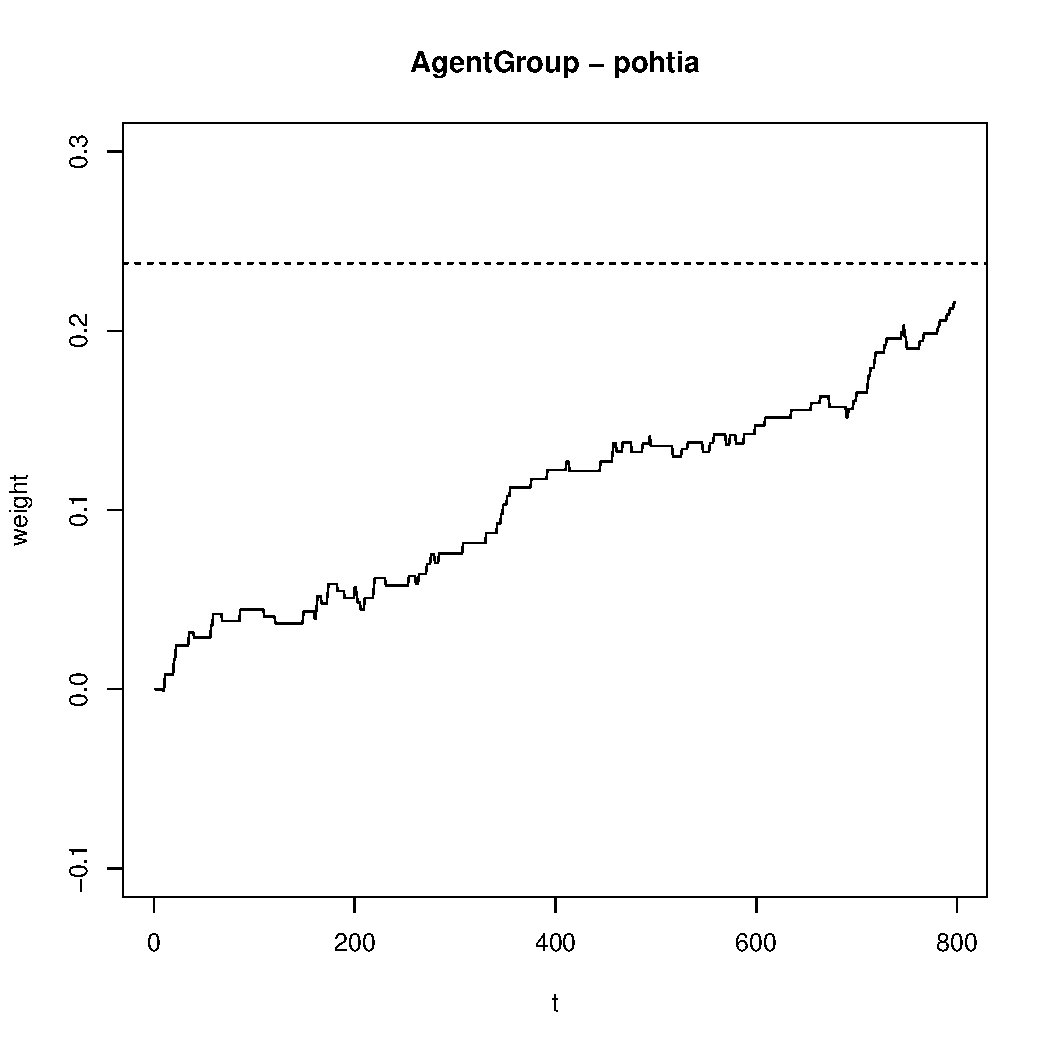
\includegraphics[width=8cm]{{{img/think.qitl1.AgentGroup_pohtia_RW_vs_D}}}}%
  \only<beamer:2| handout:0>{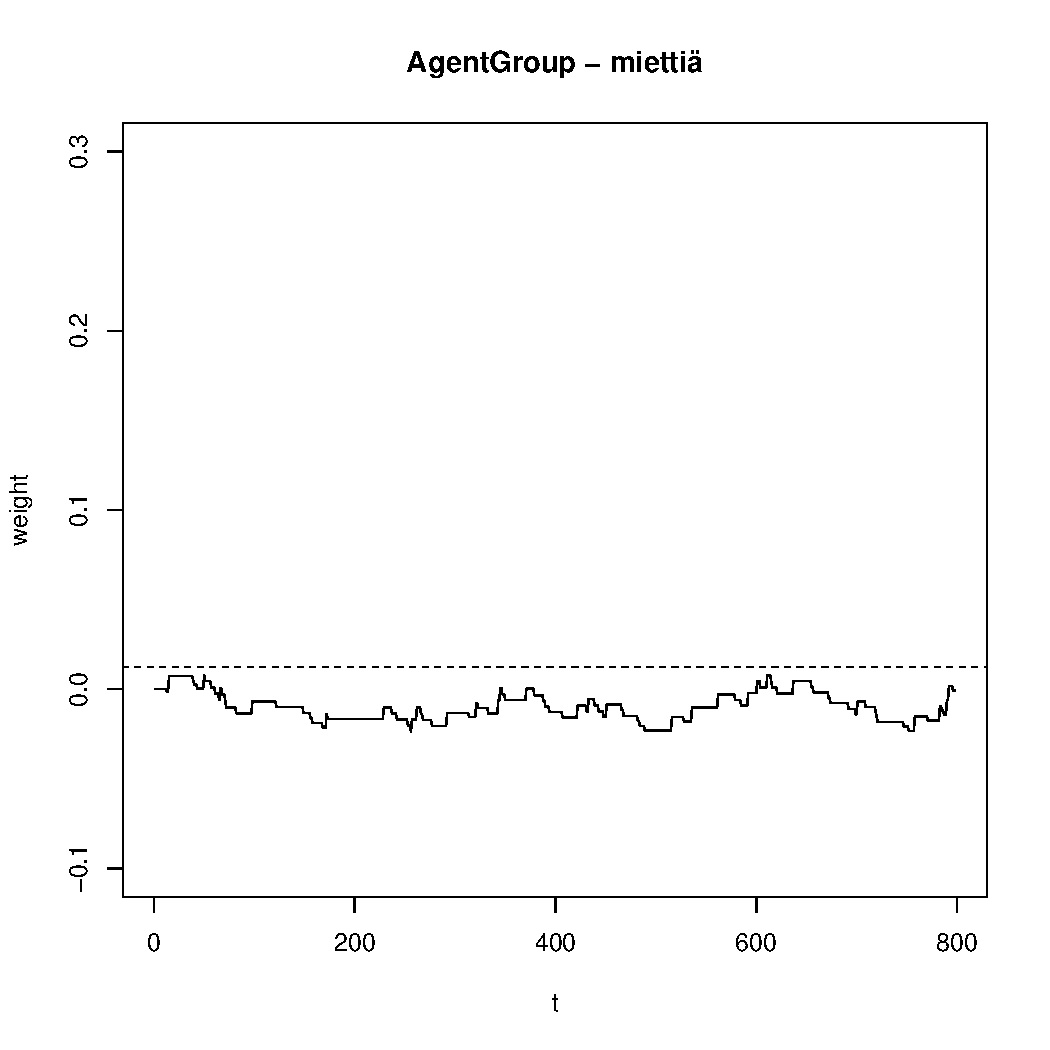
\includegraphics[width=8cm]{{{img/think.qitl1.AgentGroup_miettia_RW_vs_D}}}}%
  \only<beamer:3| handout:0>{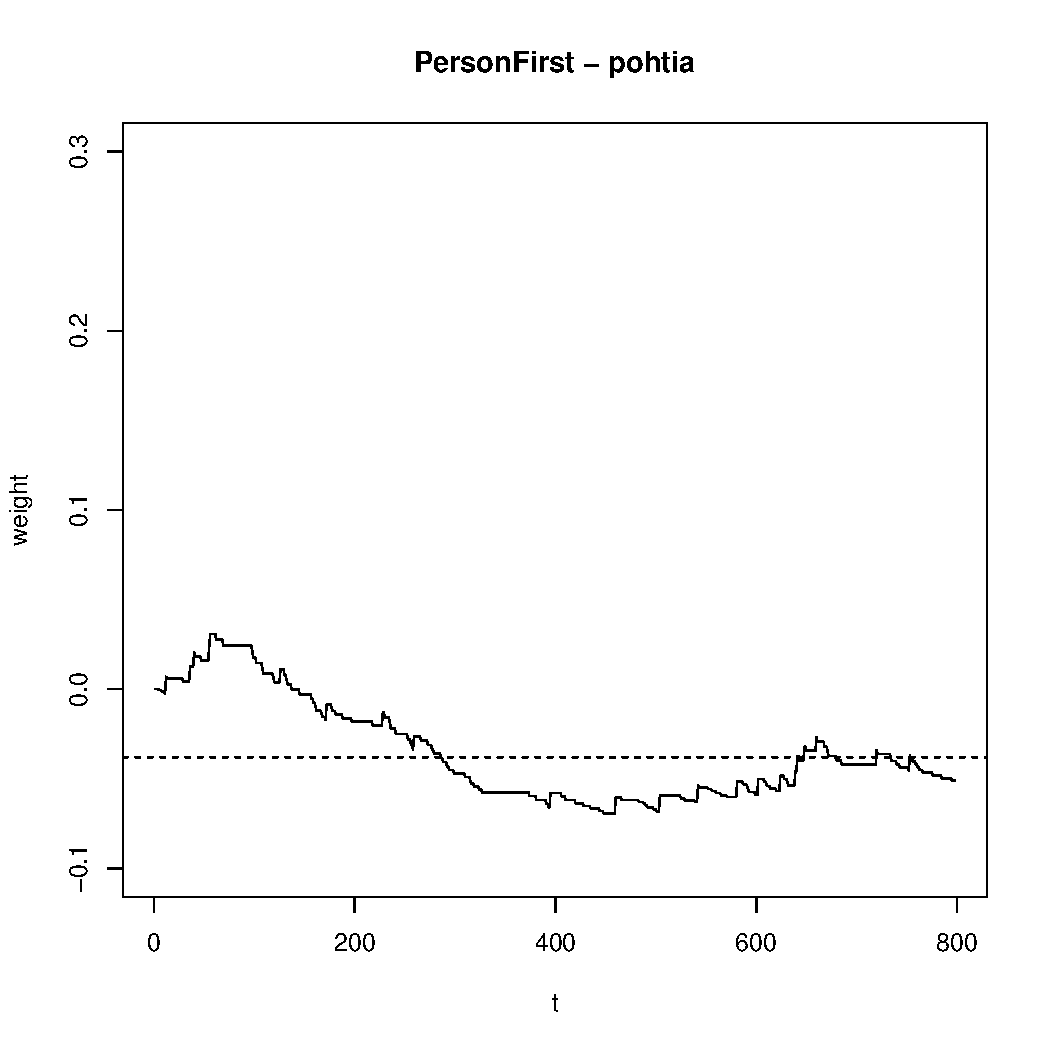
\includegraphics[width=8cm]{{{img/think.qitl1.PersonFirst_pohtia_RW_vs_D}}}}%
  \only<beamer:4| handout:0>{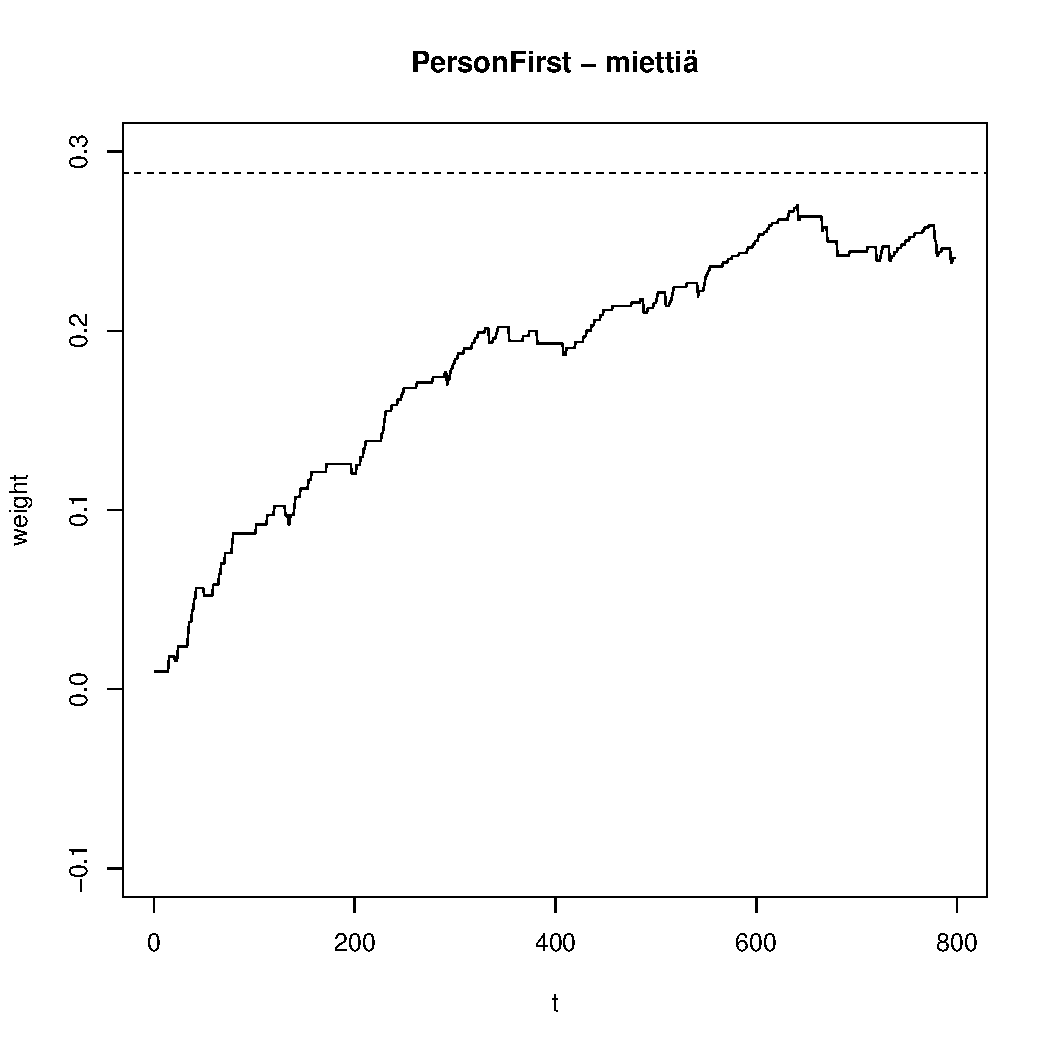
\includegraphics[width=8cm]{{{img/think.qitl1.PersonFirst_miettia_RW_vs_D}}}}%
  \only<beamer:0| handout:1>{%
    \begin{tabular}{cc}
      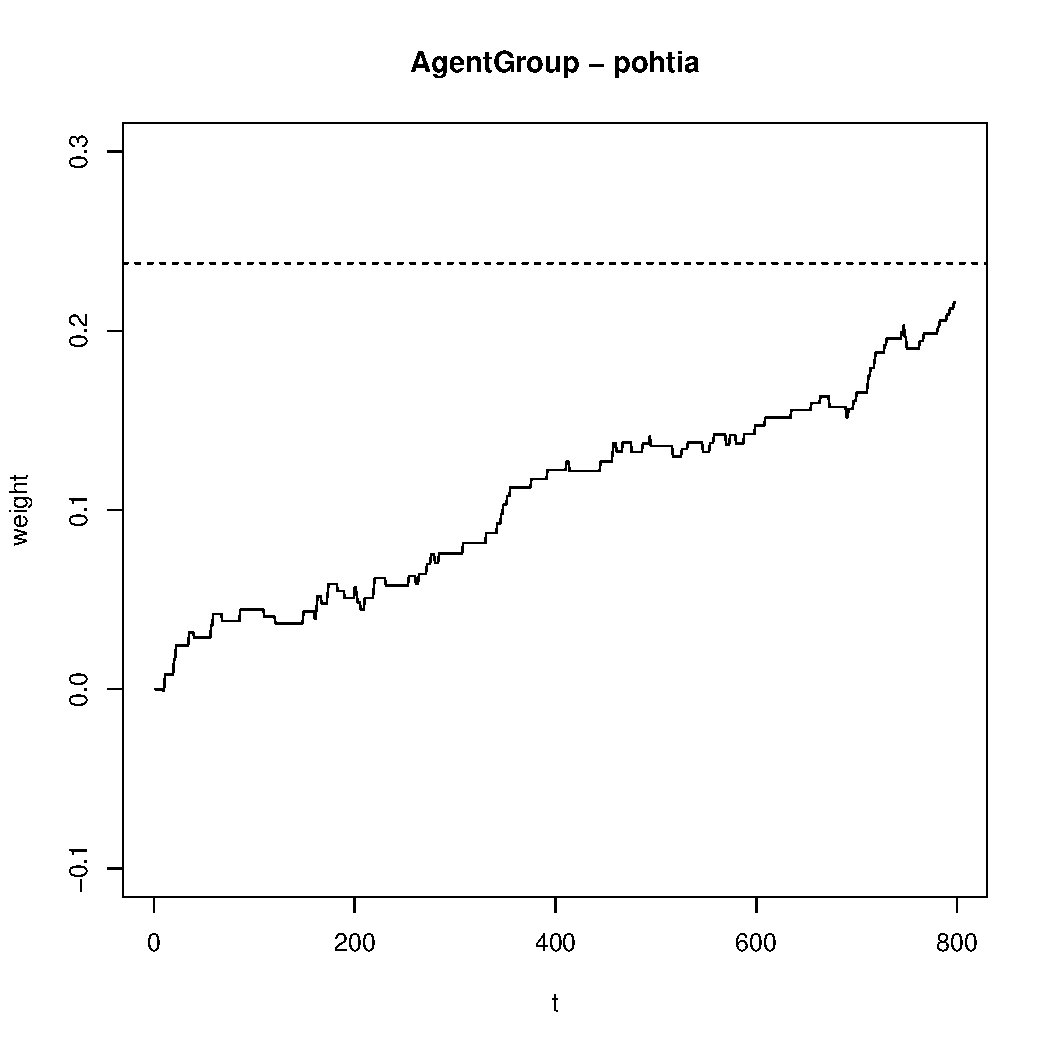
\includegraphics[width=4cm]{{{img/think.qitl1.AgentGroup_pohtia_RW_vs_D}}} &
      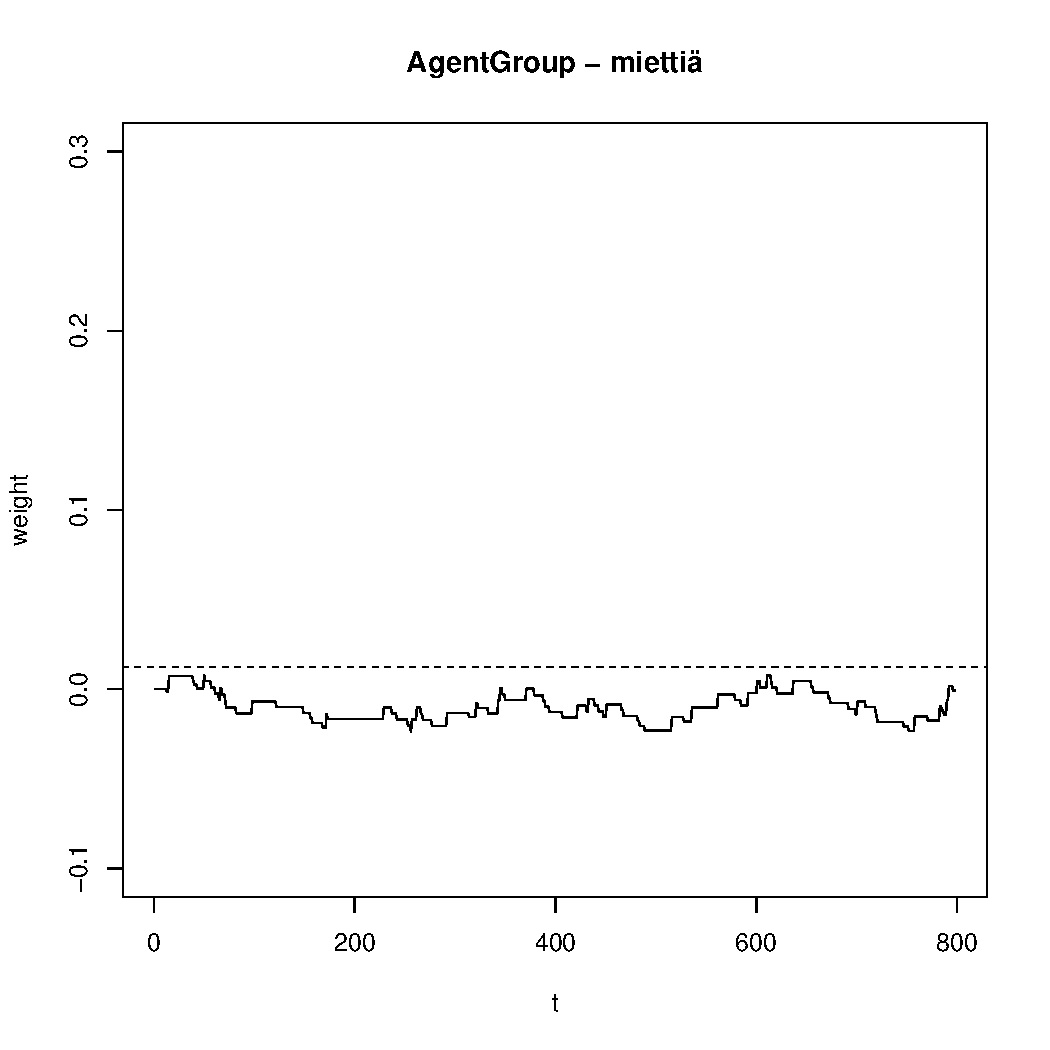
\includegraphics[width=4cm]{{{img/think.qitl1.AgentGroup_miettia_RW_vs_D}}} \\
      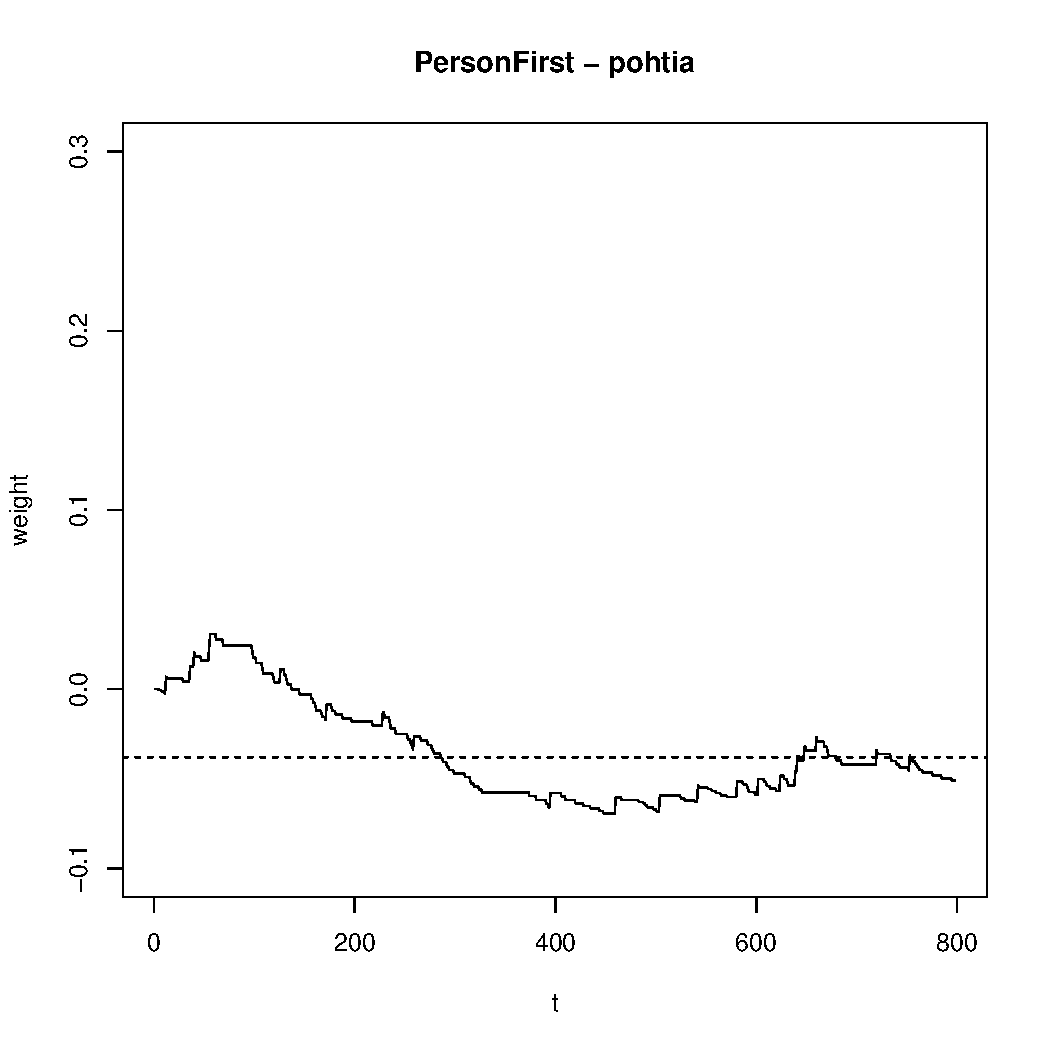
\includegraphics[width=4cm]{{{img/think.qitl1.PersonFirst_pohtia_RW_vs_D}}} &
      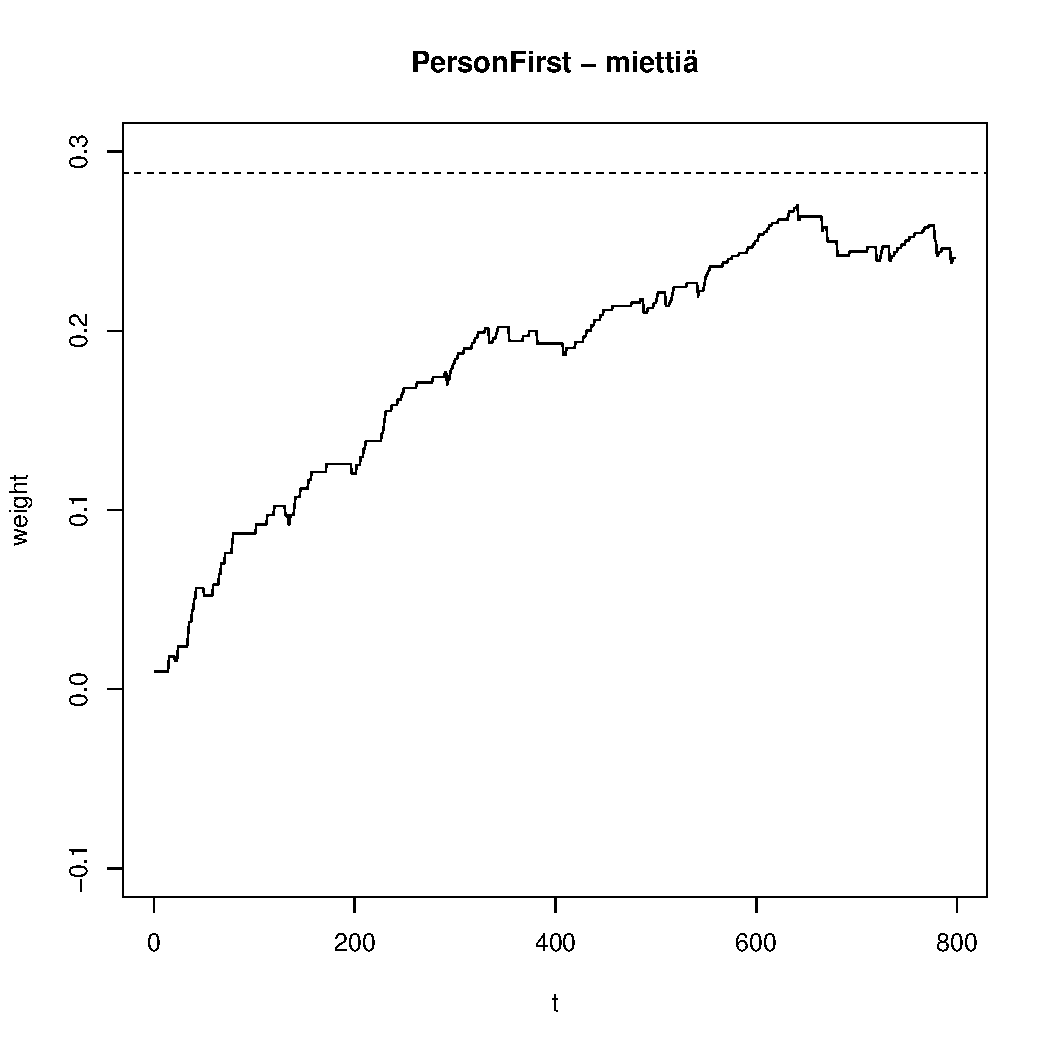
\includegraphics[width=4cm]{{{img/think.qitl1.PersonFirst_miettia_RW_vs_D}}} \\
    \end{tabular}}%
\end{frame}

\begin{frame}[c]
  \frametitle{QITL-1 through the lens of QITL-6}
  \framesubtitle{(courtesy of Dagmar Divjak)}

  \centering\ungap[2]
  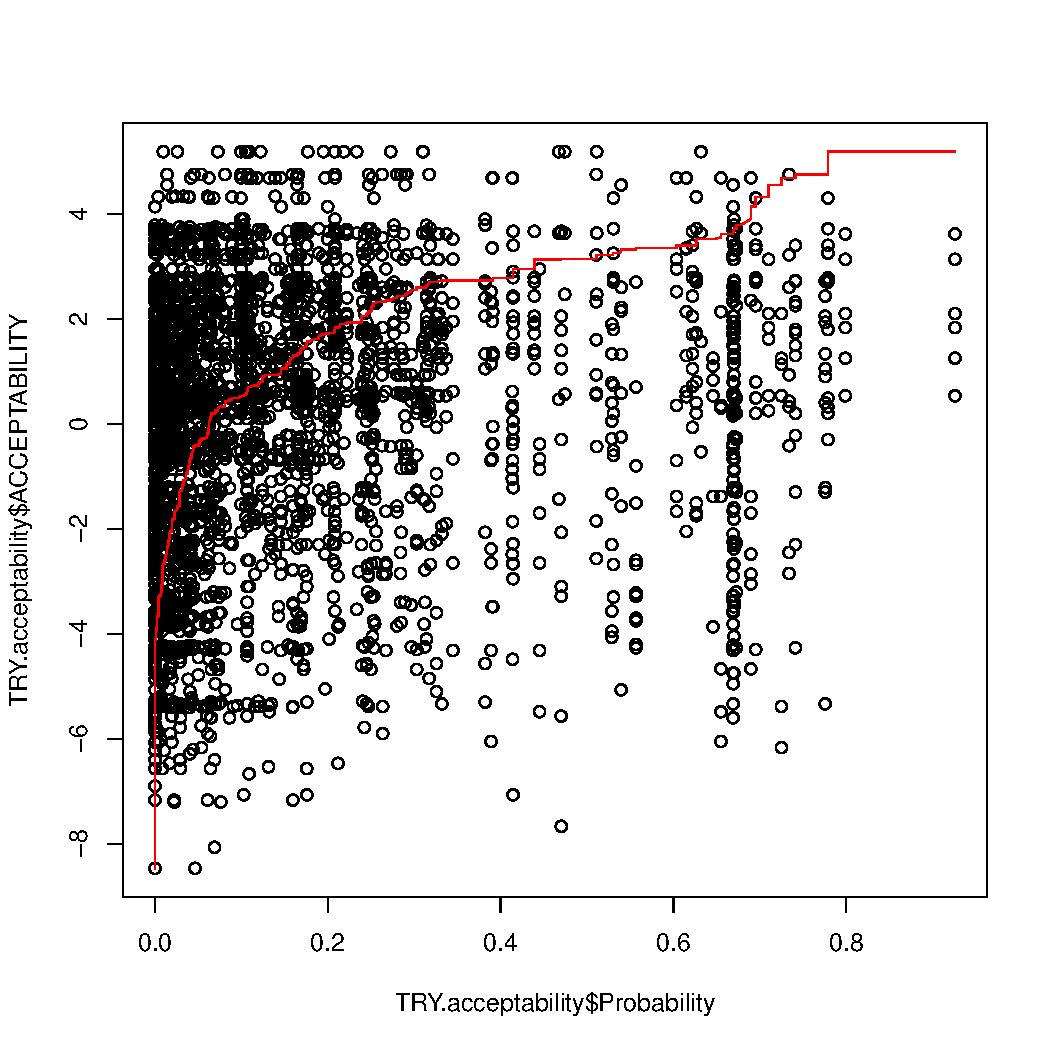
\includegraphics[width=8cm]{{{img/TRY.ACCEPTABILITY_vs_Probability}}}
\end{frame}

\begin{frame}[c]
  \frametitle{Simple \vs complex settings -- QITL-2 revisited}

  \centering
  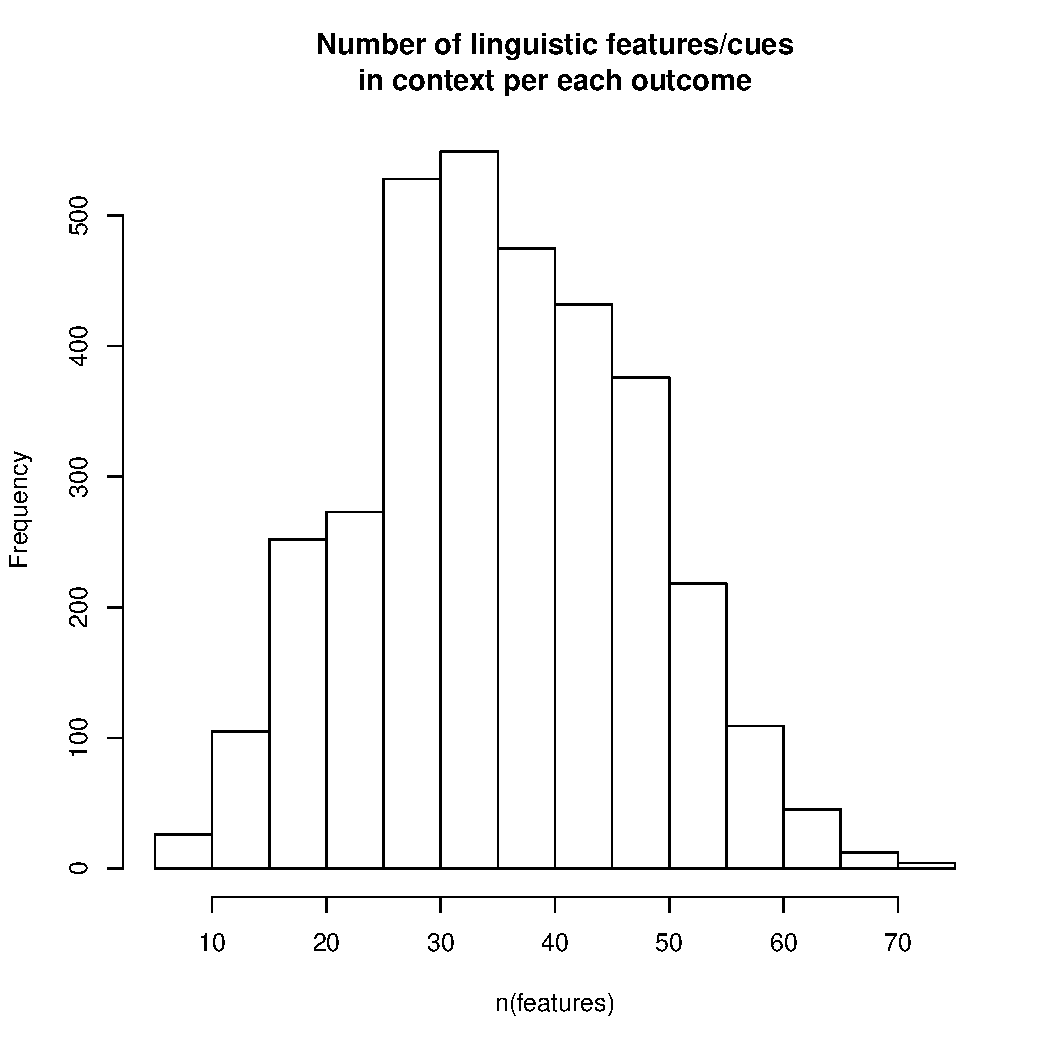
\includegraphics[width=7cm]{{{img/THINK.maximal_linguistic_variable_density}}}
\end{frame}

\begin{frame}
  \frametitle{QITL-4 revisited -- NDL \vs statistical classifiers}

  \begin{center}
    \footnotesize
    \begin{tabular}{lrrr}
      \hline
      & $\lambda_{\mbox{\tiny prediction}}$ & $\tau_{\mbox{\tiny classification}}$ & accuracy \\ 
      \hline
      Polytomous logistic regression & 0.368 & 0.488 & \textbf{0.645} \\
      (One-vs-rest) &  &  &  \\ 
      Polytomous mixed logistic regression &  &  &  \\ 
      (Poisson reformulation) &  &  &  \\ 
      $\quad\bullet$ 1$|$Section & 0.360 & 0.482 & 0.640 \\
      $\quad\bullet$ 1$|$Author & 0.358 & 0.481 & 0.640 \\
      $\quad\bullet$ 1$|$Section + 1|Author & 0.358 & 0.481 & 0.640 \\
      Support Vector Machine & 0.340 & 0.466 & 0.629 \\
      Memory-Based Learning & 0.286 & 0.422 & 0.599 \\
      (TiMBL) &  &  &  \\
      Random Forests & 0.326 & 0.455 & 0.621 \\
      Naive Discriminative Learning & 0.346 & 0.471 & \primary{0.632} \\
      \hline
    \end{tabular}
  \end{center}
  
  \scriptsize
  \secondary{Table:} Classification diagnostics for models fitted to the Finnish data set ($n=3404$). 
\end{frame}

%%% Local Variables: 
%%% mode: latex
%%% TeX-master: "../qitl6_evert_arppe"
%%% End: 


%%%%%%%%%%%%%%%%%%%%%%%%%%%%%%%%%%%%%%%%%%%%%%%%%%%%%%%%%%%%%%%%%%%%%%
%% 2 Mathematics

\section{Mathematics}

\subsection{The Rescorla-Wagner equations}

\begin{frame}
  \frametitle{The Rescorla-Wagner equations}
  %% \framesubtitle{}

  \begin{itemize}
  \item<1-> Goal of naïve discriminative learner: predict an \primary{outcome} $O$ based on presence or absence of a set of \primary{cues} $C_1, \ldots, C_n$
  \item<2-> An \primary{event} $(\vc, o)$ is formally described by indicator variables
    \begin{align*}
      c_i &= 
       \begin{cases}
         1 & \text{if $C_i$ is present} \\
         0 & \text{otherwise}
       \end{cases}
      &
      o &= 
       \begin{cases}
         1 & \text{if $O$ results} \\
         0 & \text{otherwise}
       \end{cases}
    \end{align*}
  \item<3-> Given cue-outcome \primary{associations} $\vv = (V_1, \ldots, V_n)$ of learner, the \primary{activation level} of the outcome $O$ is
    \[
    \only<beamer:3| handout:1>{
      \sum_{j=1}^n c_j V_j}
    \only<beamer:4-| handout:0>{
      \sum_{j=1}^n c_j\psupt V_j\psupt}
    \]
  \item<4-> Associations $\vv[t]$ as well as cue and outcome indicators $(\vc[t], o\psupt)$ depend on time step $t$
  \end{itemize}
\end{frame}

\begin{frame}
  \frametitle{The Rescorla-Wagner equations}
  %% \framesubtitle{}
  
  \begin{itemize}
  \item \citet{Rescorla:Wagner:72} proposed the \primary{R-W equations} for the change in associations given an event $(\vc, o)$:
    \[
    \Delta V_i =
    \begin{cases}
      0 & \text{if } c_i = 0\\
      \alpha_i \beta_1 \bigl(\lambda - \sum_{j=1}^n c_j V_j \bigr) & \text{if } c_i = 1 \wedge o = 1 \\
      \alpha_i \beta_2 \bigl(0 - \sum_{j=1}^n c_j V_j \bigr) & \text{if } c_i = 1 \wedge o = 0 
    \end{cases}
    \]
    with parameters
    \ungap[.5]
    \begin{align*}
      \lambda &> 0   && \text{target activation level for outcome $O$} \\
      \alpha_i &> 0  && \text{salience of cue $C_i$} \\
      \beta_1 &> 0   && \text{learning rate for positive ovents ($o = 1$)} \\
      \beta_2 &> 0   && \text{learning rate for negative ovents ($o = 0$)}
    \end{align*}
  \end{itemize}
\end{frame}

\begin{frame}<beamer:1-3| handout:1>
  \frametitle{The Widrow-Hoff rule}
  %% \framesubtitle{}
  
  \begin{itemize}
  \item The \primary{W-H rule} \citep{Widrow:Hoff:60} is a widely-used simplification of the R-W equations:
    \begin{align*}
    \Delta V_i &=
    \begin{cases}
      0 & \text{if } c_i = 0\\
      \only<beamer:1| handout:0>{\alpha_i} \beta\only<beamer:1| handout:0>{_1} \bigl(\only<beamer:1| handout:0>{\lambda}\only<beamer:2-| handout:1>{1} - \sum_{j=1}^n c_j V_j \bigr) & \text{if } c_i = 1 \wedge o = 1 \\
      \only<beamer:1| handout:0>{\alpha_i} \beta\only<beamer:1| handout:0>{_2} \bigl(0 - \sum_{j=1}^n c_j V_j \bigr) & \text{if } c_i = 1 \wedge o = 0 
    \end{cases}
    \only<beamer:3-| handout:1>{\\
       &= \primary{c_i \beta \bigl( o - \textstyle\sum_{j=1}^n c_j V_j \bigr)}}
    \end{align*}
    with parameters
    \ungap[.5]
    \begin{align*}
      \lambda  &= 1   && \text{target activation level for outcome $O$} \\
      \alpha_i &= 1  && \text{salience of cue $C_i$} \\
      \beta_1  &= \beta_2   && \text{global learning rate for positive and}\\
               &= \beta > 0 && \text{negative events}
    \end{align*}
  \end{itemize}
\end{frame}

\begin{frame}[c]
  \frametitle{A simple example: German noun plurals}
  %% \framesubtitle{}
  
  \small\centering
  \begin{tabular}{r>{\color{counterpoint}}l|c|cccccc}
    \toprule
    $t$ & & $o$ & $c_1$ & $c_2$ & $c_3$ & $c_4$ & $c_5$ & $c_6$ \\
    & \secondary{word} & \secondary{pl?} & \secondary{\emph{--e}} & \secondary{\emph{--n}} & \secondary{\emph{--s}} & \secondary{umlaut} & \secondary{dbl cons} & \secondary{bgrd}\\
    \midrule
    1 &   Bäume &  1  &  1 & 0 & 0 & 1 & 0 & 1 \\ 
    2 & Flasche &  0  &  1 & 0 & 0 & 0 & 0 & 1 \\ 
    3 &    Baum &  0  &  0 & 0 & 0 & 0 & 0 & 1 \\ 
    4 &  Gläser &  1  &  0 & 0 & 0 & 1 & 0 & 1 \\ 
    5 &Flaschen &  1  &  0 & 1 & 0 & 0 & 0 & 1 \\ 
    6 &   Latte &  0  &  1 & 0 & 0 & 0 & 1 & 1 \\ 
    7 &  Hütten &  1  &  0 & 1 & 0 & 1 & 1 & 1 \\ 
    8 &    Glas &  0  &  0 & 0 & 1 & 0 & 0 & 1 \\ 
    9 &   Bäume &  1  &  1 & 0 & 0 & 1 & 0 & 1 \\ 
   10 &    Füße &  1  &  1 & 0 & 0 & 1 & 0 & 1 \\
    \bottomrule
  \end{tabular}
\end{frame}

\begin{frame}[c]
  \frametitle{A simple example: German noun plurals}
  %% \framesubtitle{}
  
  \footnotesize\centering
  \begin{tabular}{>{\color{counterpoint}}c|c|cccccc}
    \toprule
    \secondary{$t$} & \secondary{$\sum c_j V_j$} & \secondary{$V_1$} & \secondary{$V_2$} & \secondary{$V_3$} & \secondary{$V_4$} & \secondary{$V_5$} & \secondary{$V_6$} \\
\only<beamer:1| handout:0>{\color{foreground}  1 & .000 & .000 & .000 &  .000 & .000 &  .000 & .000 }% 
\only<beamer:2| handout:0>{\color{foreground}  2 & .400 & .200 & .000 &  .000 & .200 &  .000 & .200 }% 
\only<beamer:3| handout:0>{\color{foreground}  3 & .120 & .120 & .000 &  .000 & .200 &  .000 & .120 }% 
\only<beamer:4| handout:0>{\color{foreground}  4 & .296 & .120 & .000 &  .000 & .200 &  .000 & .096 }% 
\only<beamer:5| handout:0>{\color{foreground}  5 & .237 & .120 & .000 &  .000 & .341 &  .000 & .237 }% 
\only<beamer:6| handout:0>{\color{foreground}  6 & .509 & .120 & .153 &  .000 & .341 &  .000 & .389 }% 
\only<beamer:7| handout:0>{\color{foreground}  7 & .679 & .018 & .153 &  .000 & .341 & -.102 & .288 }% 
\only<beamer:8| handout:0>{\color{foreground}  8 & .352 & .018 & .217 &  .000 & .405 & -.038 & .352 }% 
\only<beamer:9| handout:0>{\color{foreground}  9 & .704 & .018 & .217 & -.070 & .405 & -.038 & .281 }% 
\only<beamer:10| handout:1>{\color{foreground}10 & .882 & .077 & .217 & -.070 & .464 & -.038 & .340 }% 
\only<beamer:11| handout:0>{\color{foreground}11 &      & .101 & .217 & -.070 & .488 & -.038 & .364 }%
    \\
    \midrule
    \only<beamer:1| handout:0>{   Bäume &  1  &  1 & 0 & 0 & 1 & 0 & 1 \\ }% 
    \only<beamer:2| handout:0>{ Flasche &  0  &  1 & 0 & 0 & 0 & 0 & 1 \\ }% 
    \only<beamer:3| handout:0>{    Baum &  0  &  0 & 0 & 0 & 0 & 0 & 1 \\ }% 
    \only<beamer:4| handout:0>{  Gläser &  1  &  0 & 0 & 0 & 1 & 0 & 1 \\ }% 
    \only<beamer:5| handout:0>{Flaschen &  1  &  0 & 1 & 0 & 0 & 0 & 1 \\ }% 
    \only<beamer:6| handout:0>{   Latte &  0  &  1 & 0 & 0 & 0 & 1 & 1 \\ }% 
    \only<beamer:7| handout:0>{  Hütten &  1  &  0 & 1 & 0 & 1 & 1 & 1 \\ }% 
    \only<beamer:8| handout:0>{    Glas &  0  &  0 & 0 & 1 & 0 & 0 & 1 \\ }% 
    \only<beamer:9| handout:0>{   Bäume &  1  &  1 & 0 & 0 & 1 & 0 & 1 \\ }% 
    \only<beamer:10| handout:1>{   Füße &  1  &  1 & 0 & 0 & 1 & 0 & 1 \\}% 
    \only<beamer:11| handout:0>{& & & & & & & \\ }%
    \phantom{Flaschen} & \secondary{$o$} & \secondary{$c_1$} & \secondary{$c_2$} & \secondary{$c_3$} & \secondary{$c_4$} & \secondary{$c_5$} & \secondary{$c_6$} \\
    \bottomrule
  \end{tabular}

  \gap[1]
  \only<beamer:1| handout:0>{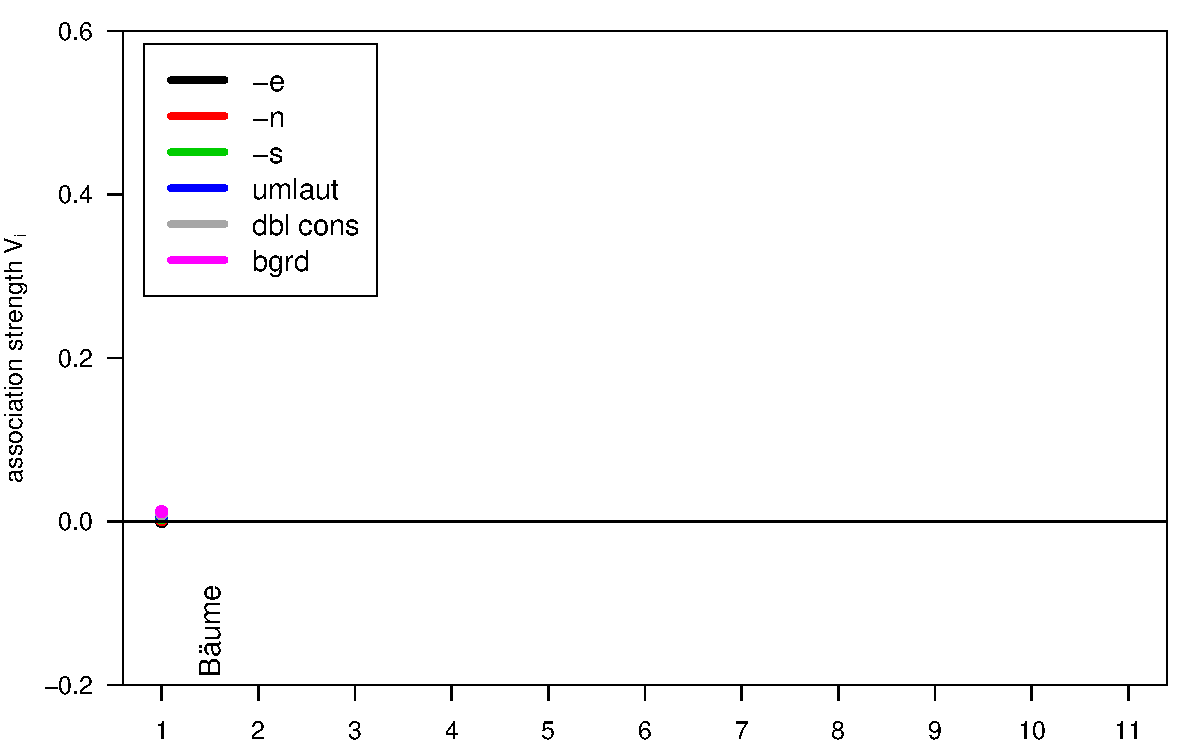
\includegraphics[width=8cm]{img/german_plural_rw_step_1}}%
  \only<beamer:2| handout:0>{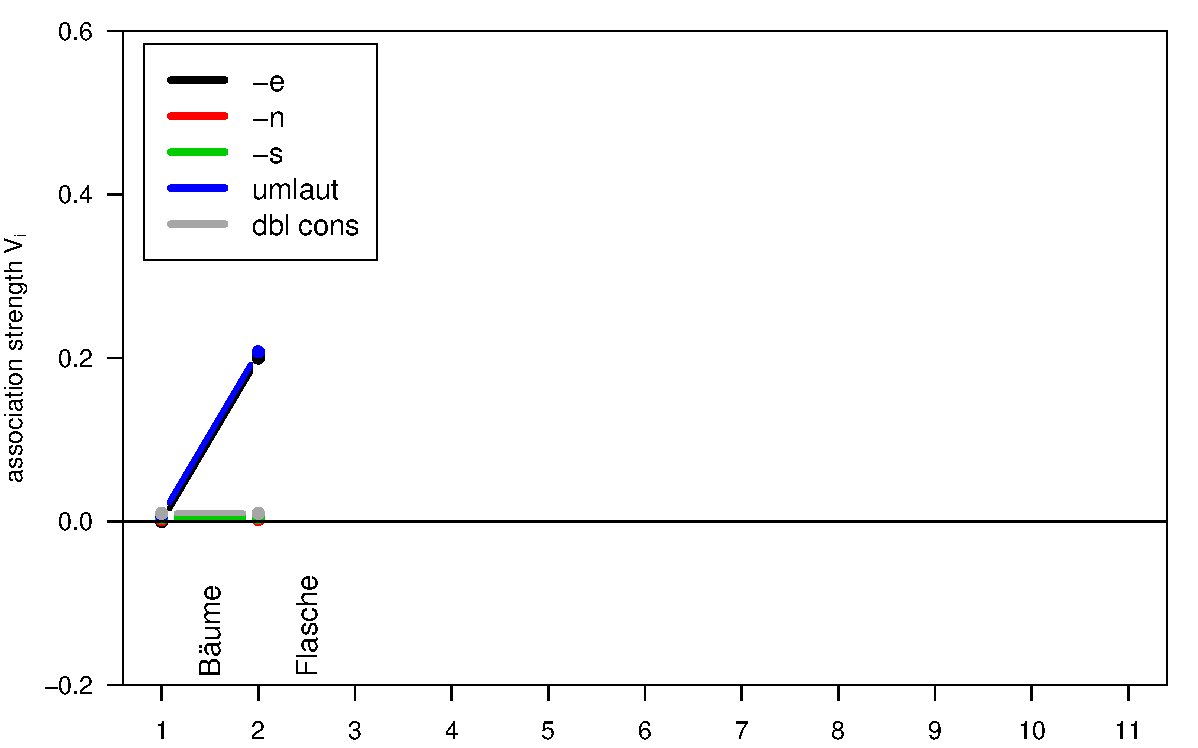
\includegraphics[width=8cm]{img/german_plural_rw_step_2}}%
  \only<beamer:3| handout:0>{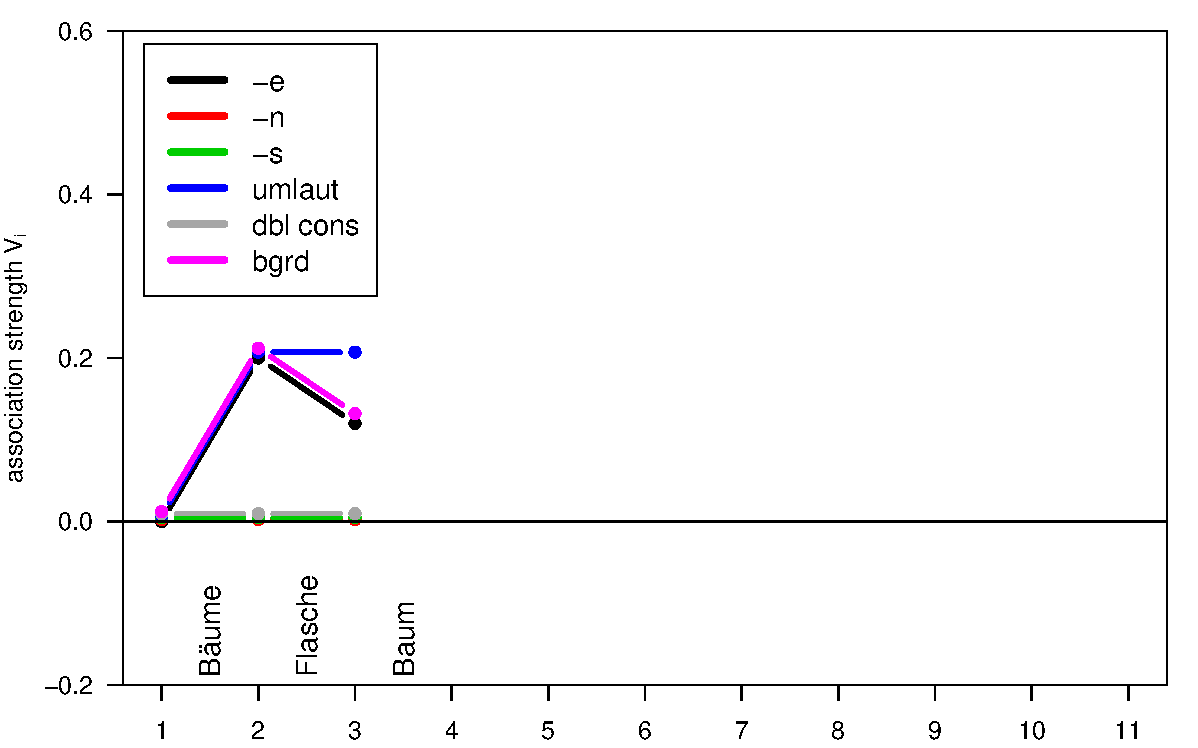
\includegraphics[width=8cm]{img/german_plural_rw_step_3}}%
  \only<beamer:4| handout:0>{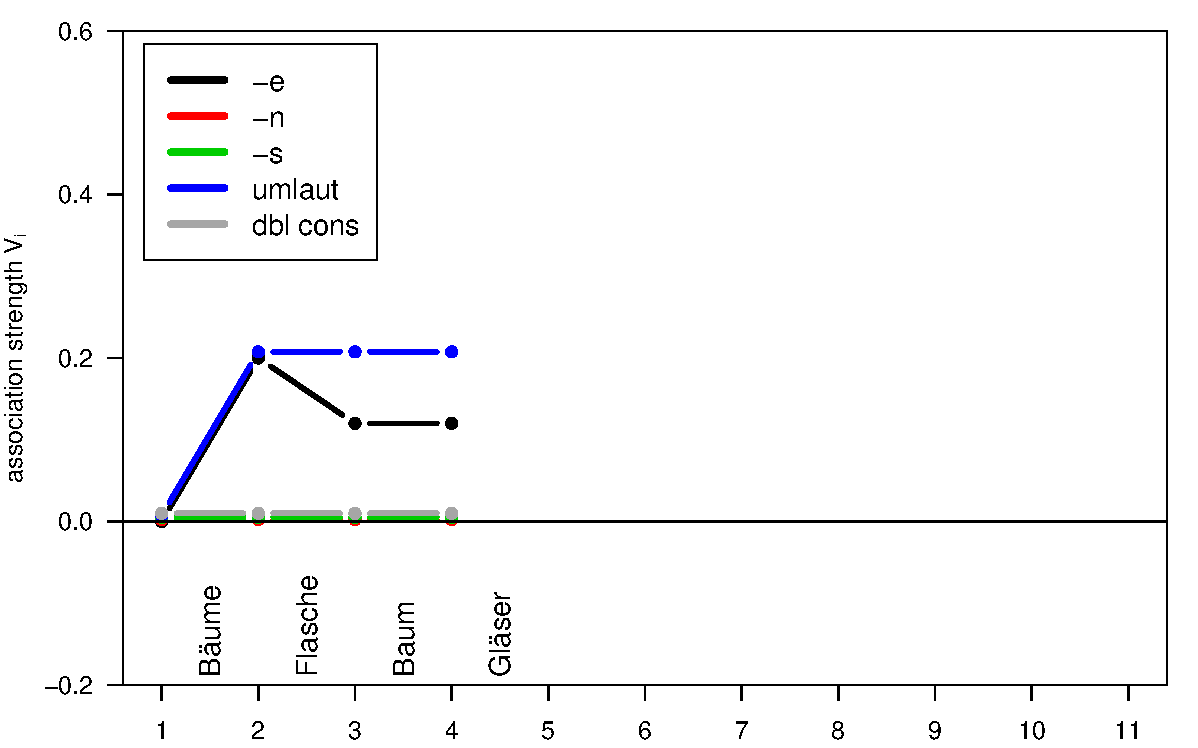
\includegraphics[width=8cm]{img/german_plural_rw_step_4}}%
  \only<beamer:5| handout:0>{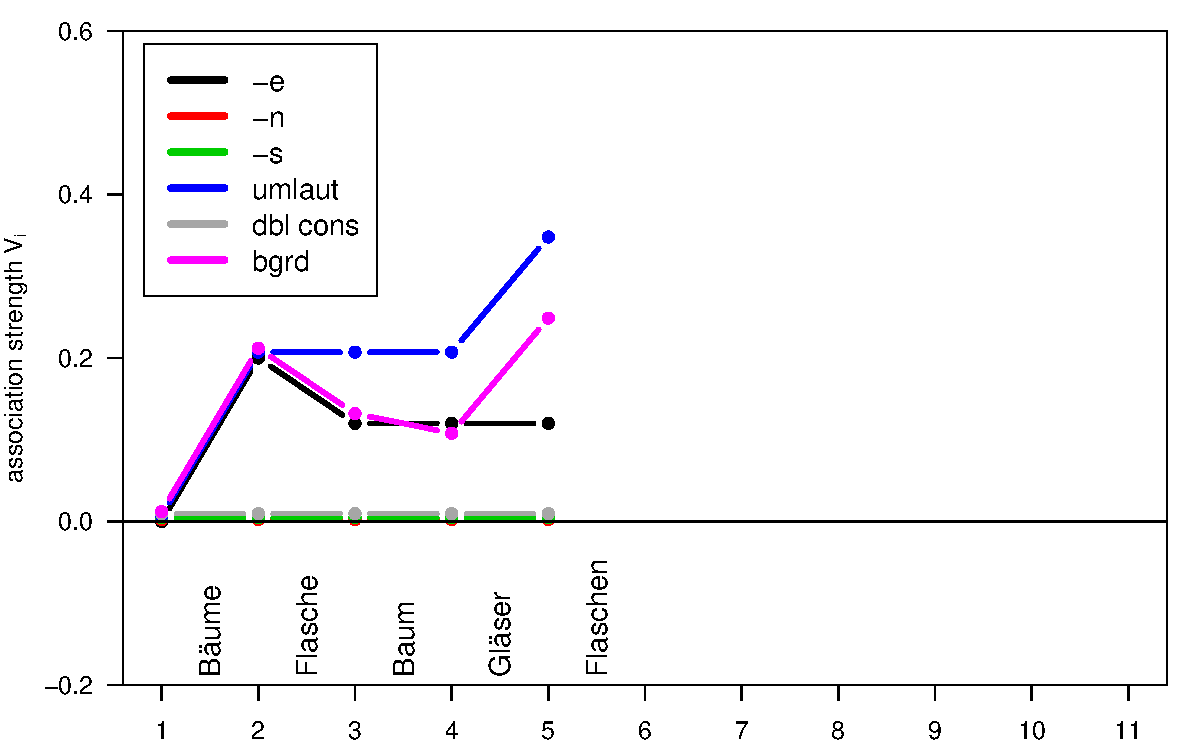
\includegraphics[width=8cm]{img/german_plural_rw_step_5}}%
  \only<beamer:6| handout:0>{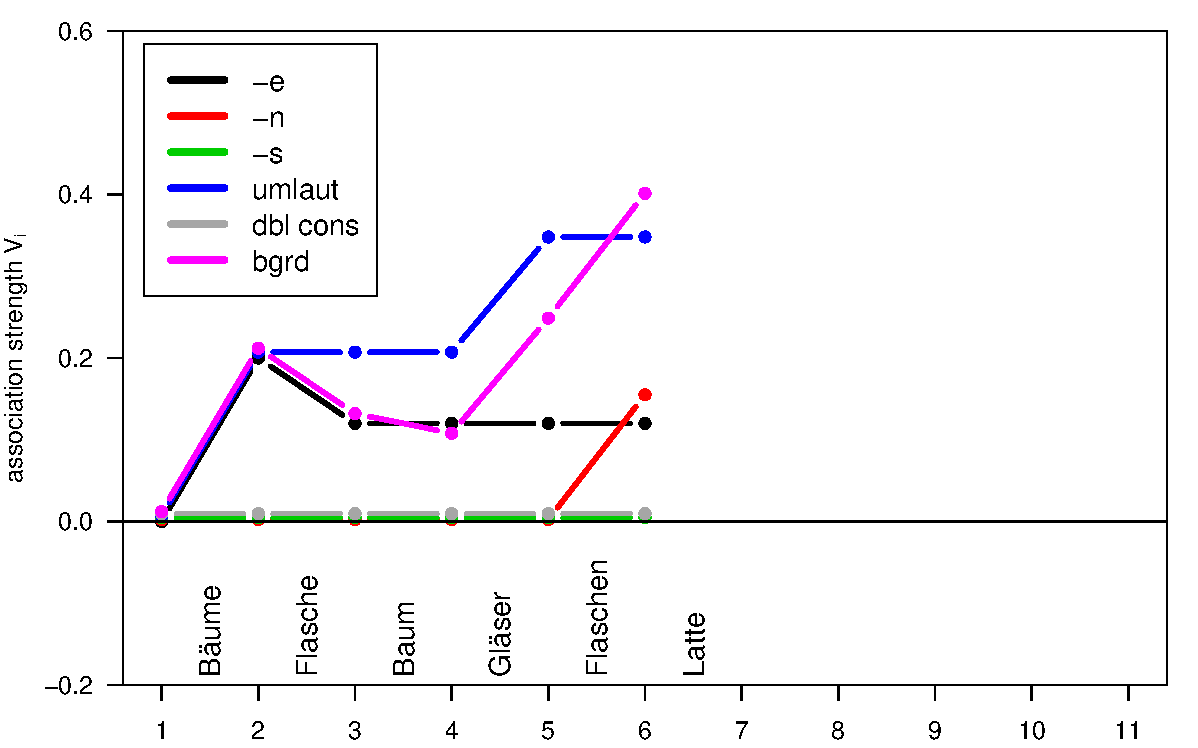
\includegraphics[width=8cm]{img/german_plural_rw_step_6}}%
  \only<beamer:7| handout:0>{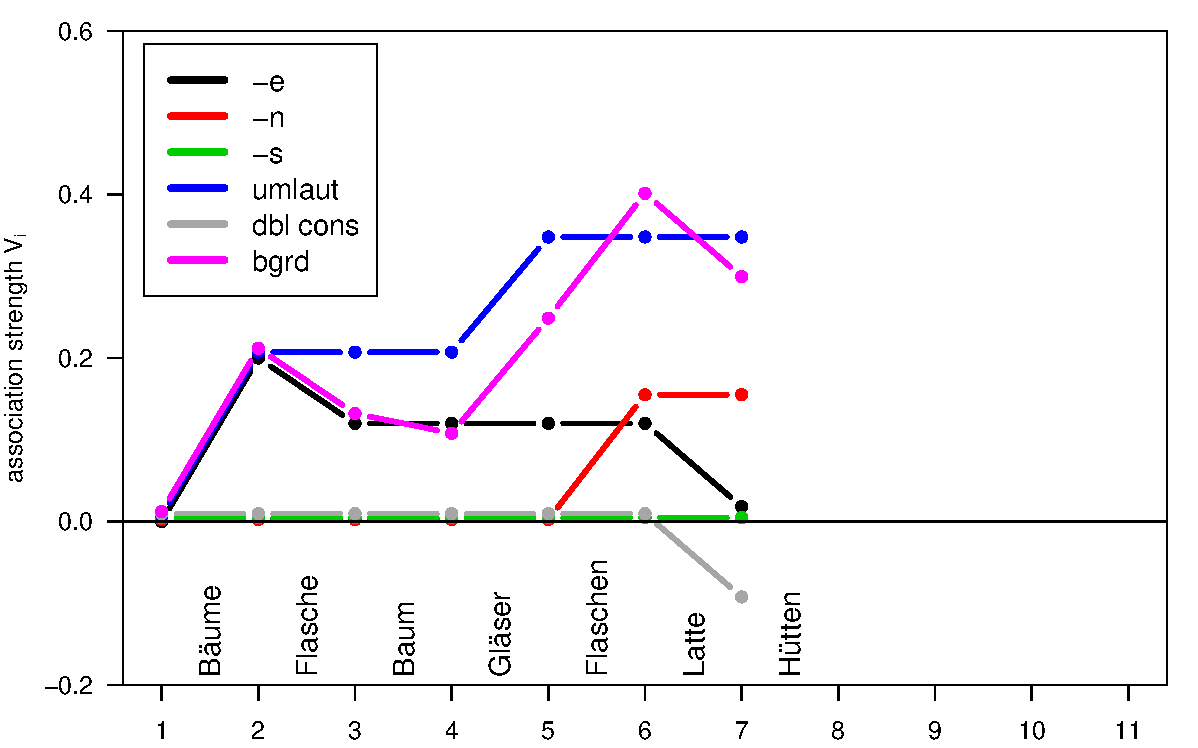
\includegraphics[width=8cm]{img/german_plural_rw_step_7}}%
  \only<beamer:8| handout:0>{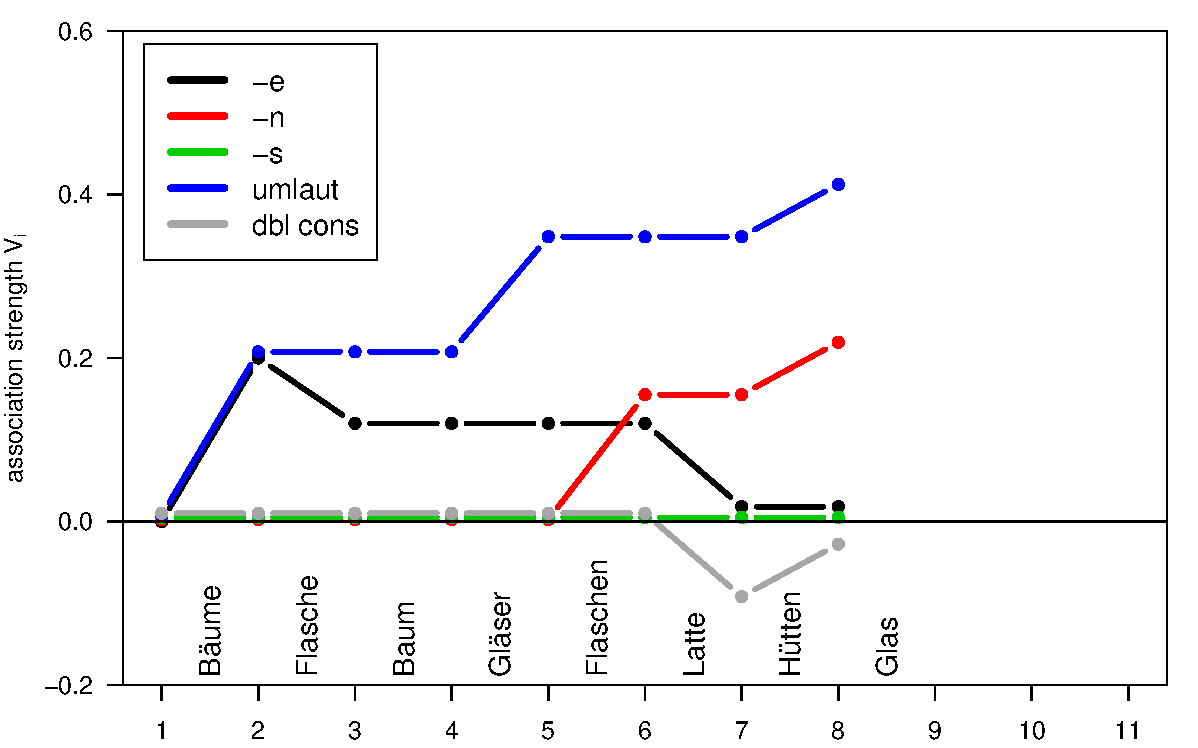
\includegraphics[width=8cm]{img/german_plural_rw_step_8}}%
  \only<beamer:9| handout:0>{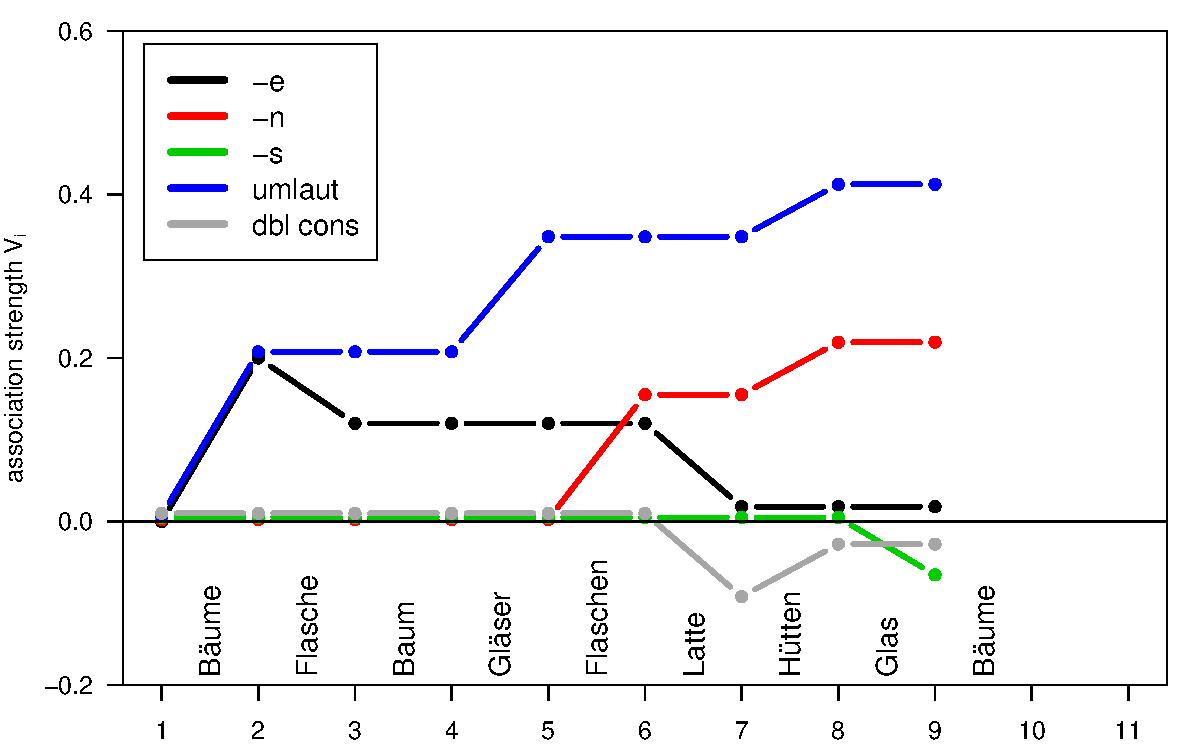
\includegraphics[width=8cm]{img/german_plural_rw_step_9}}%
  \only<beamer:10| handout:1>{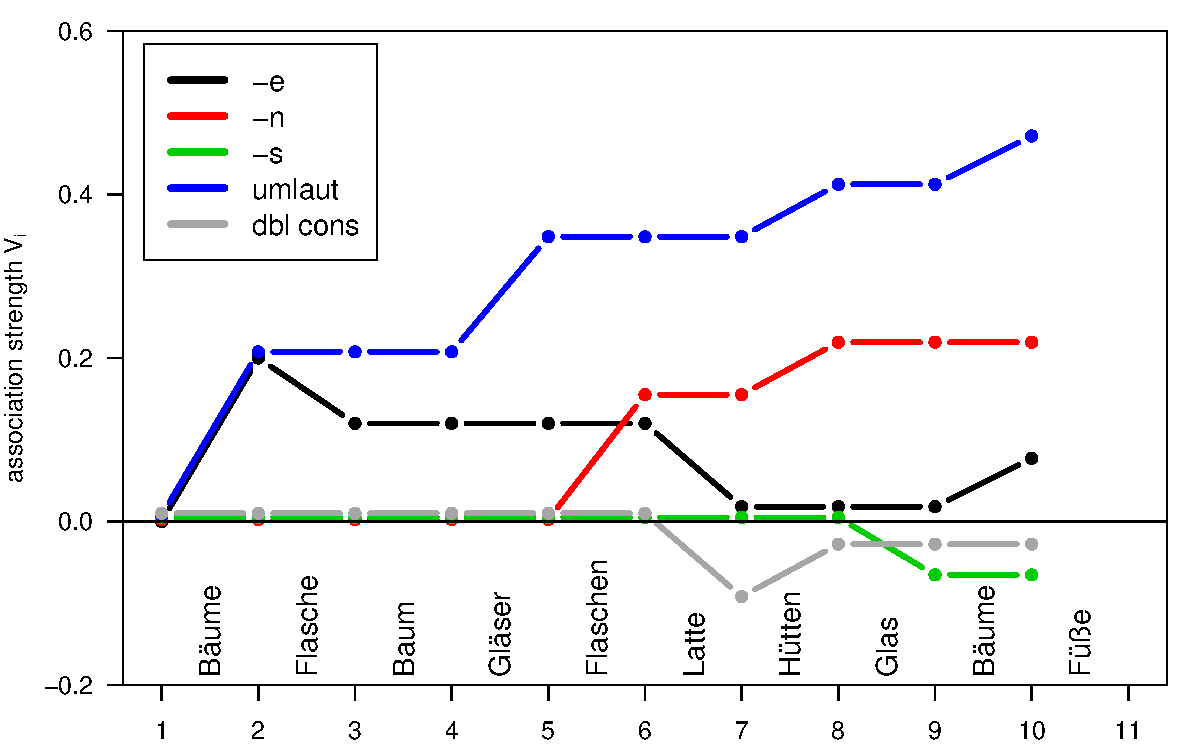
\includegraphics[width=8cm]{img/german_plural_rw_step_10}}%
  \only<beamer:11| handout:0>{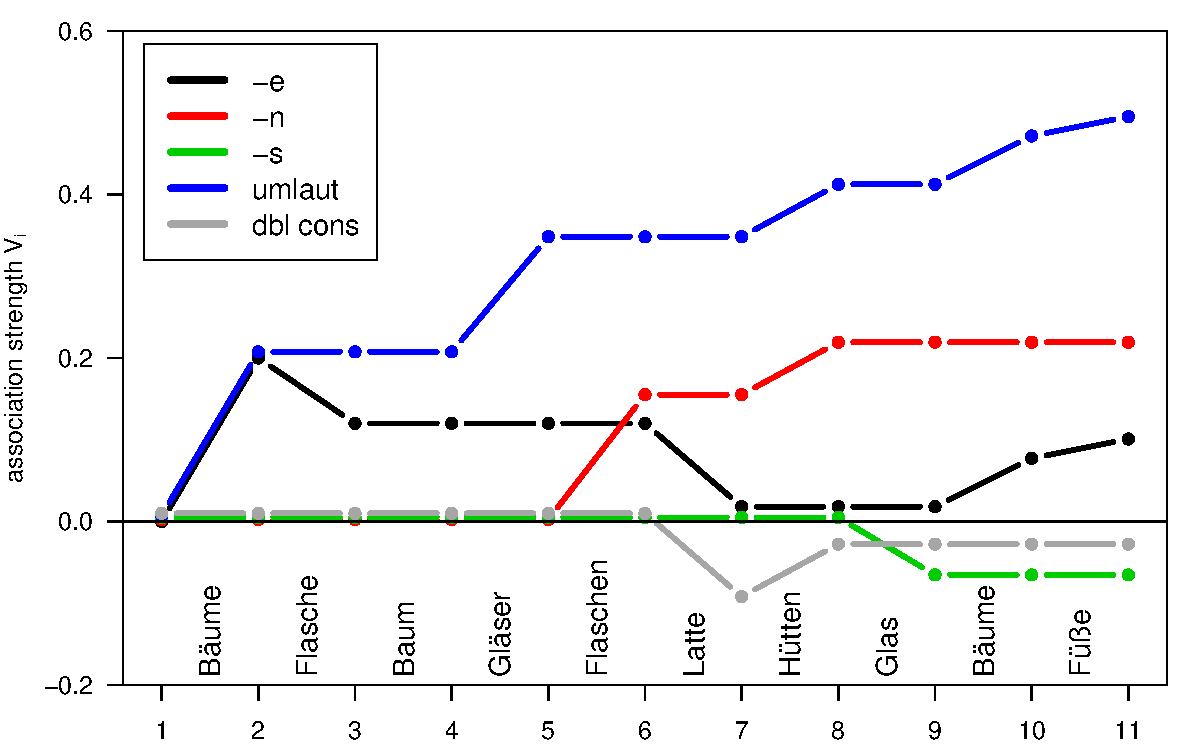
\includegraphics[width=8cm]{img/german_plural_rw_step_11}}%
\end{frame}

\begin{frame}
  \frametitle{A stochastic NDL learner}
  %% \framesubtitle{}

  \begin{itemize}
  \item<1-> A specific event sequence $(\vc[t], o\psupt)$ will only be encountered in controlled experiments
  \item<2-> For applications in corpus linguistics, it is more plausible to assume that events are randomly sampled from a population of \primary{event tokens} $(\vc[k], o\psup{k})$ for $k = 1, \ldots, m$
    \begin{itemize}
    \item[\hand] event types listed repeatedly proportional to their frequency
    \end{itemize}
  \item<3-> I.i.d.\ random variables $\vc[t] \sim \vc$ and $o\psupt\sim o$
    \begin{itemize}
    \item[\hand] distributions of $\vc$ and $o$ determined by population
    \end{itemize}
  \item<3-> NDL can now be trained for arbitrary number of time steps, even if population is small (as in our example)
    \begin{itemize}
    \item study asymptotic behaviour of learners
    \item convergence \so stable ``adult'' state of associations
    \end{itemize}
  \end{itemize}
\end{frame}

\begin{frame}[c]
  \frametitle{A stochastic NDL learner}
  \framesubtitle{Effect of the learning rate $\beta$}

  \centering\ungap[1]
  \only<beamer:1| handout:1>{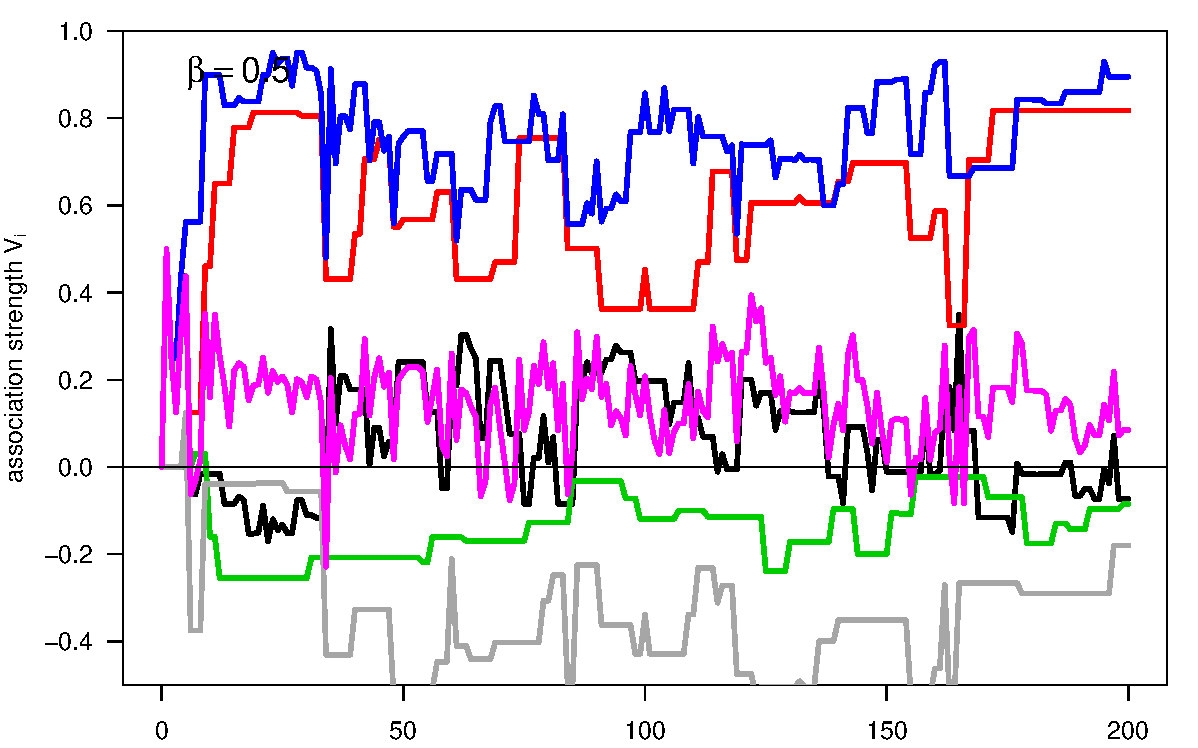
\includegraphics[width=11cm]{img/german_plural_rw_b050_n200}}%
  \only<beamer:2| handout:0>{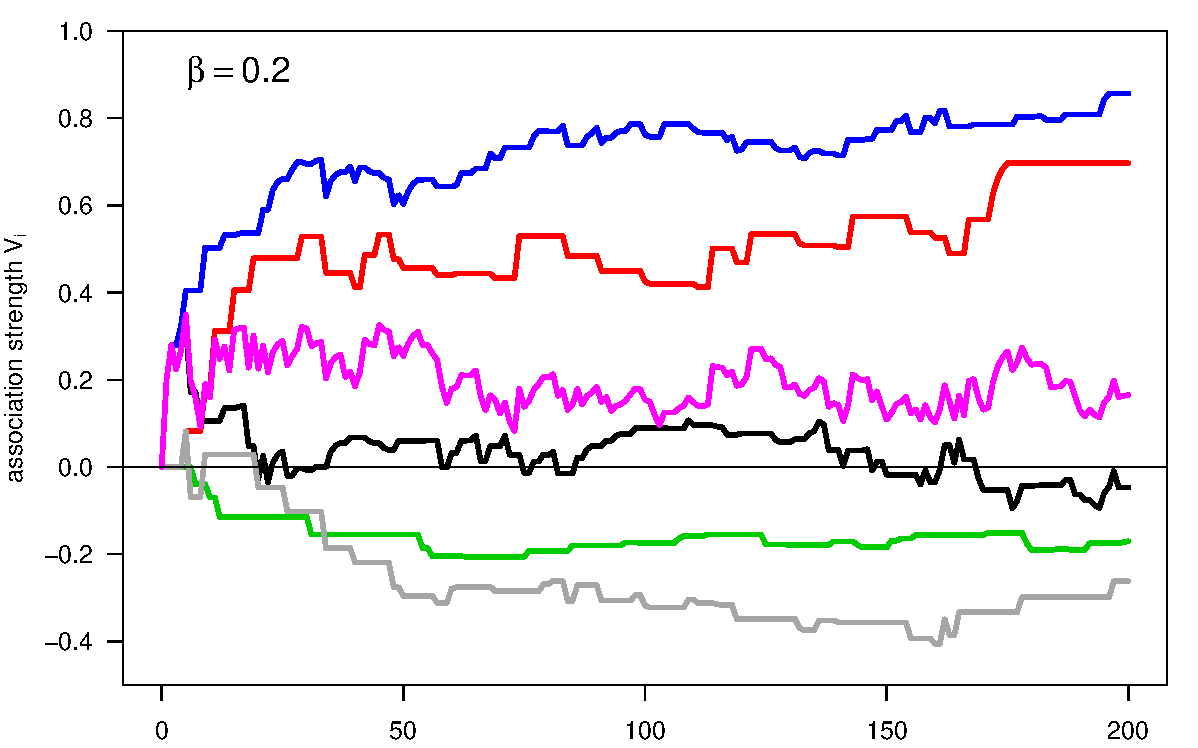
\includegraphics[width=11cm]{img/german_plural_rw_b020_n200}}%
  \only<beamer:3| handout:0>{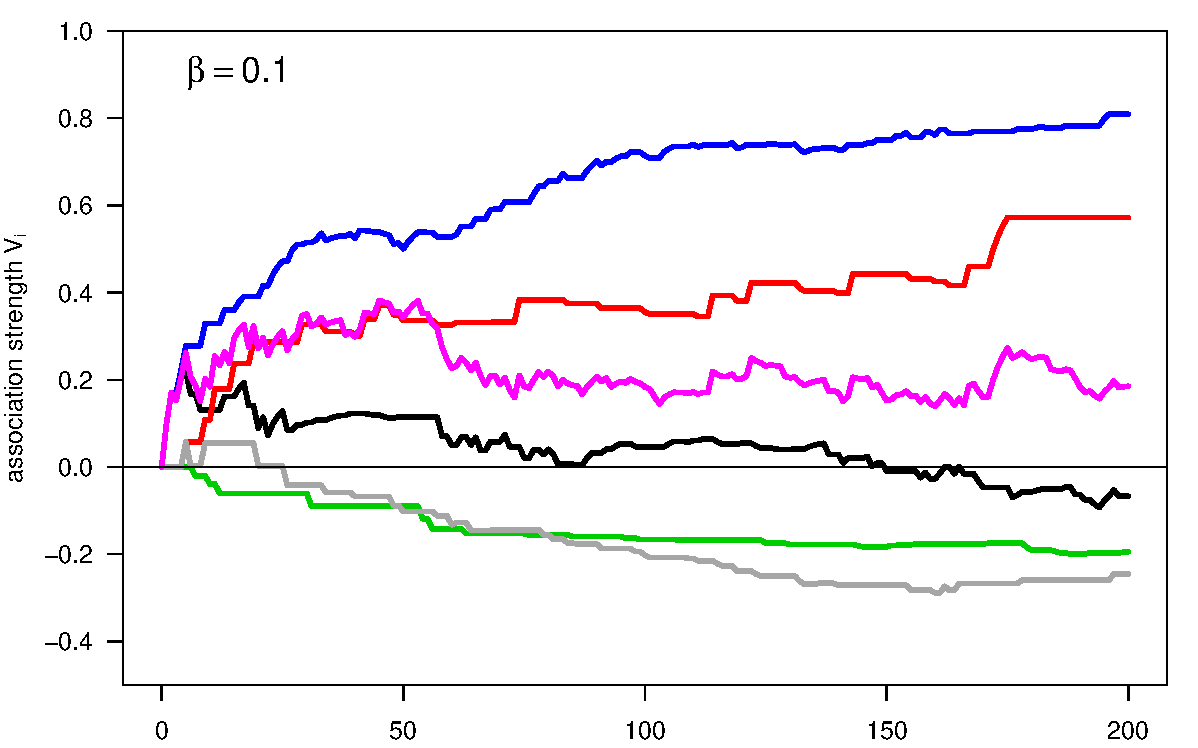
\includegraphics[width=11cm]{img/german_plural_rw_b010_n200}}%
  \only<beamer:4| handout:1>{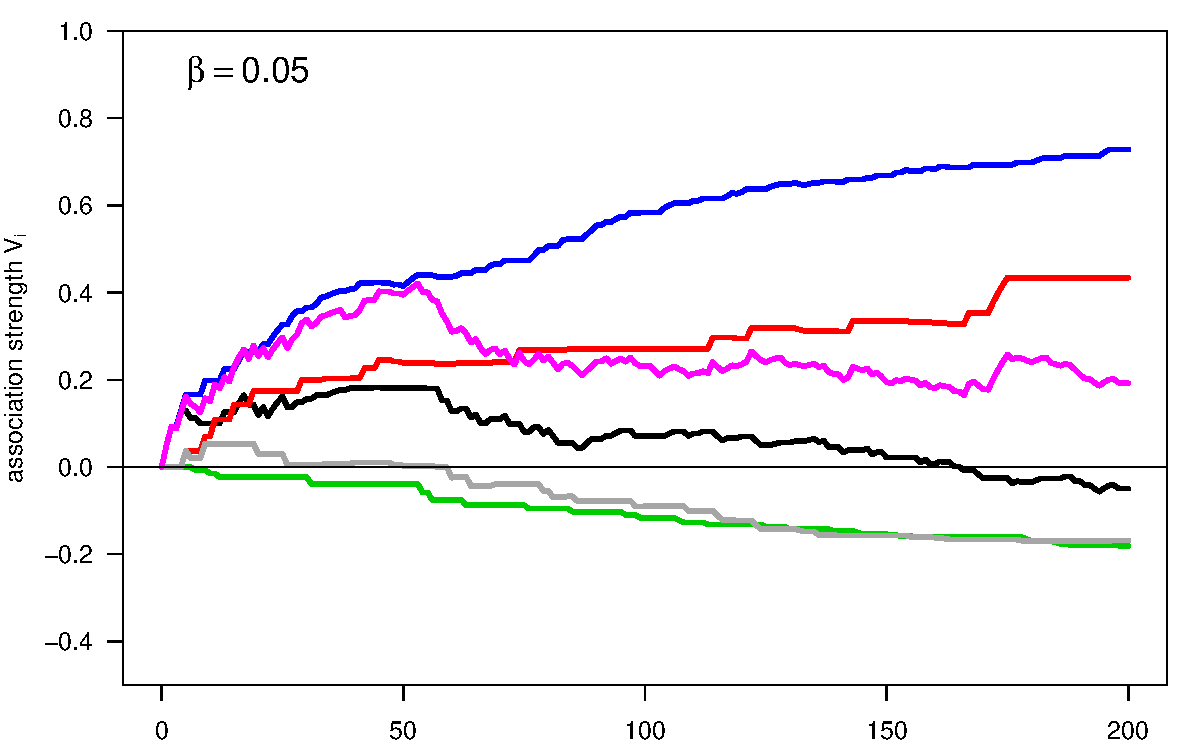
\includegraphics[width=11cm]{img/german_plural_rw_b005_n200}}%
  \only<beamer:5| handout:0>{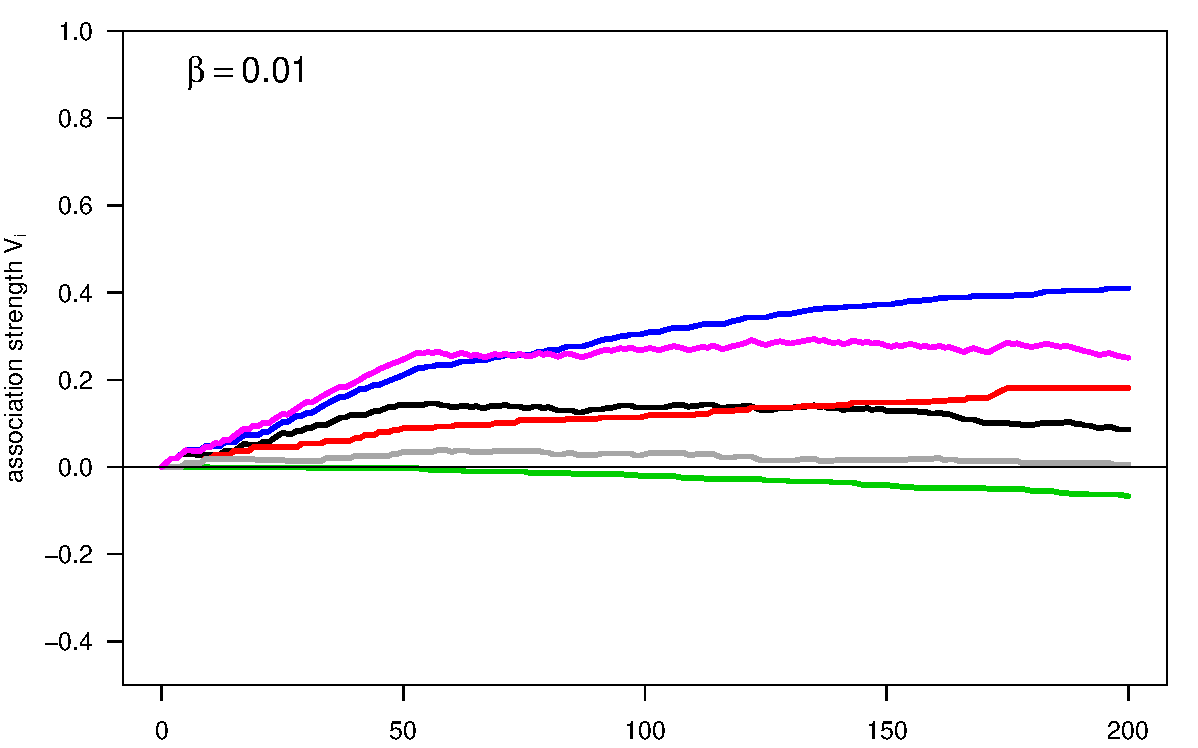
\includegraphics[width=11cm]{img/german_plural_rw_b001_n200}}%
  \only<beamer:6| handout:0>{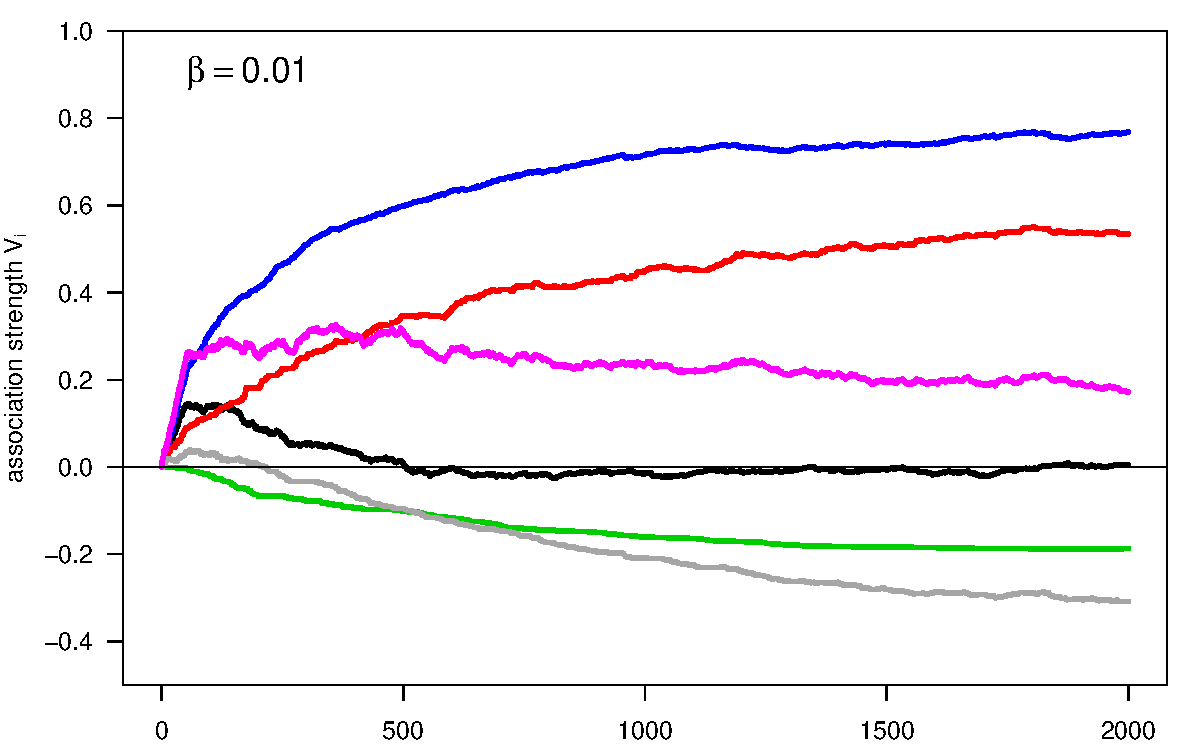
\includegraphics[width=11cm]{img/german_plural_rw_b001_n2000}}%
\end{frame}

%%% Local Variables: 
%%% mode: latex
%%% TeX-master: "../qitl6_evert_arppe"
%%% End: 


\subsection{The Danks equilibrium}

\begin{frame}
  \frametitle{Expected activation levels}
  %% \framesubtitle{}

  \begin{itemize}
  \item Since we are interested in the general behaviour of a stochastic NDL, it makes sense to average over many individual learners to obtain \primary{expected associations} $\bigExp{V_j\psupt}$
  \end{itemize}

  \[
  \bigExp{V_{j}\psup{t+1}} = \bigExp{V_j\psupt} + \bigExp{\Delta V_j\psupt}
  \]

  \ungap[.5]
  \begin{align*}
    \bigExp{\Delta V_j\psupt} 
    &= \Expscale{ 
      c_i \beta \bigl( o - \textstyle\sum_{j=1}^n c_j V_j\psupt \bigr)
      } \qquad\qquad\qquad\qquad \\
    & \only<beamer:2| handout:0>{
      = \beta\cdot \bigExp{c_i o} - \beta\cdot \Expscale{c_i \textstyle\sum_{j=1}^n c_j V_j\psupt}
      }%
      \only<beamer:3| handout:0>{
      = \beta\cdot \bigExp{c_i o} - \beta\cdot \textstyle\sum_{j=1}^n \secondary{\bigExp{c_i c_j V_j\psupt}}
      }%
      \only<beamer:4| handout:0>{
      = \beta\cdot \secondary{\bigExp{c_i o}} - \beta\cdot \textstyle\sum_{j=1}^n \secondary{\bigExp{c_i c_j}} \bigExp{V_j\psupt}
      }% 
      \only<beamer:5| handout:1>{
      = \beta\cdot\left( \p{C_i, O} - \textstyle\sum_{j=1}^n \p{C_i, C_j} \bigExp{V_j\psupt} \right)
      }% 
  \end{align*}

  \begin{itemize}
  \item<3-> $c_i$ and $c_j$ are independent from $V_j\psupt$
  \item<4-> indicator variables: $\Exp{c_i o} = \p{C_i, O}$; $\Exp{c_i c_j} = \p{C_i, C_j}$
  \end{itemize}
\end{frame}

\begin{frame}
  \frametitle{Expected activation levels}
  %% \framesubtitle{}
  
  \ungap[1.5]
  \[
  \only<beamer:1-5| handout:0>{\Delta V_j\psupt = c_i\psupt \beta \bigl( o\psupt - \textstyle\sum_{j=1}^n c_j\psupt V_j\psupt \bigr)}%
  \only<beamer:6-| handout:1>{\bigExp{\Delta V_j\psupt} = \beta\cdot\bigl( \p{C_i, O} - \textstyle\sum_{j=1}^n \p{C_i, C_j} \bigExp{V_j\psupt} \bigr)}%
  \]
  
  \centering
  \only<beamer:1| handout:0>{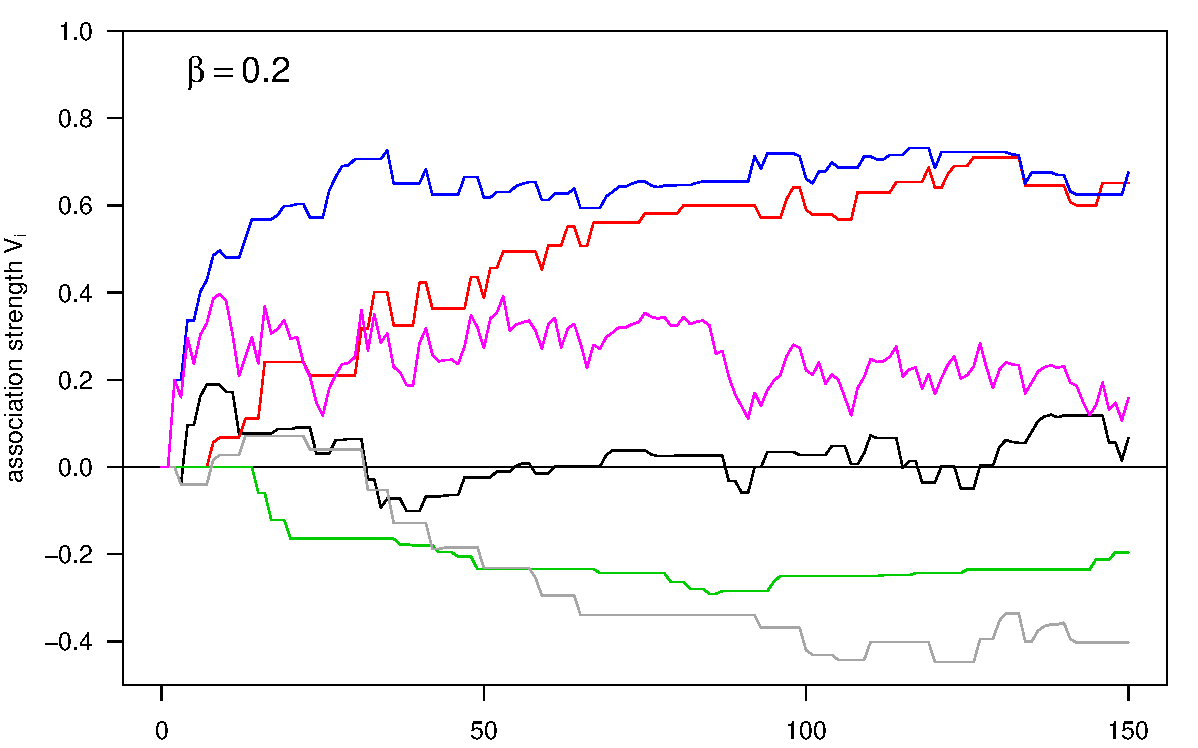
\includegraphics[width=10cm]{img/german_plural_exp_rw_step_1}}%
  \only<beamer:2| handout:0>{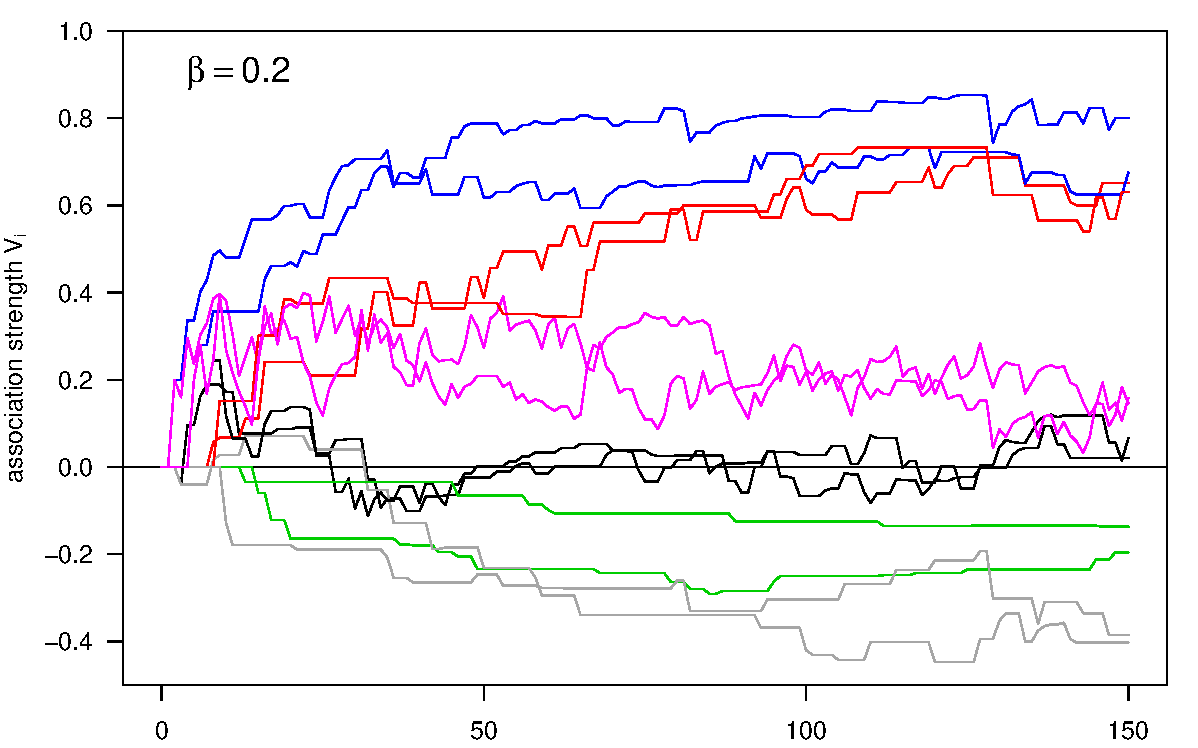
\includegraphics[width=10cm]{img/german_plural_exp_rw_step_2}}%
  \only<beamer:3| handout:0>{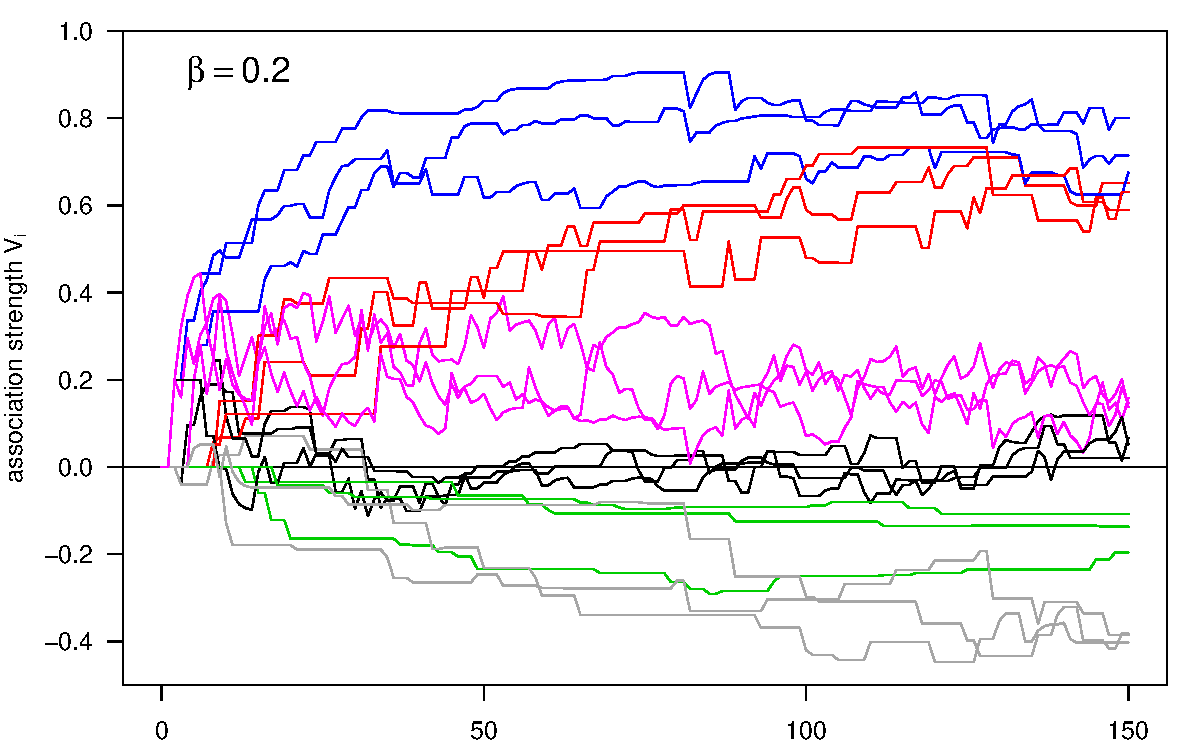
\includegraphics[width=10cm]{img/german_plural_exp_rw_step_3}}%
  \only<beamer:4| handout:0>{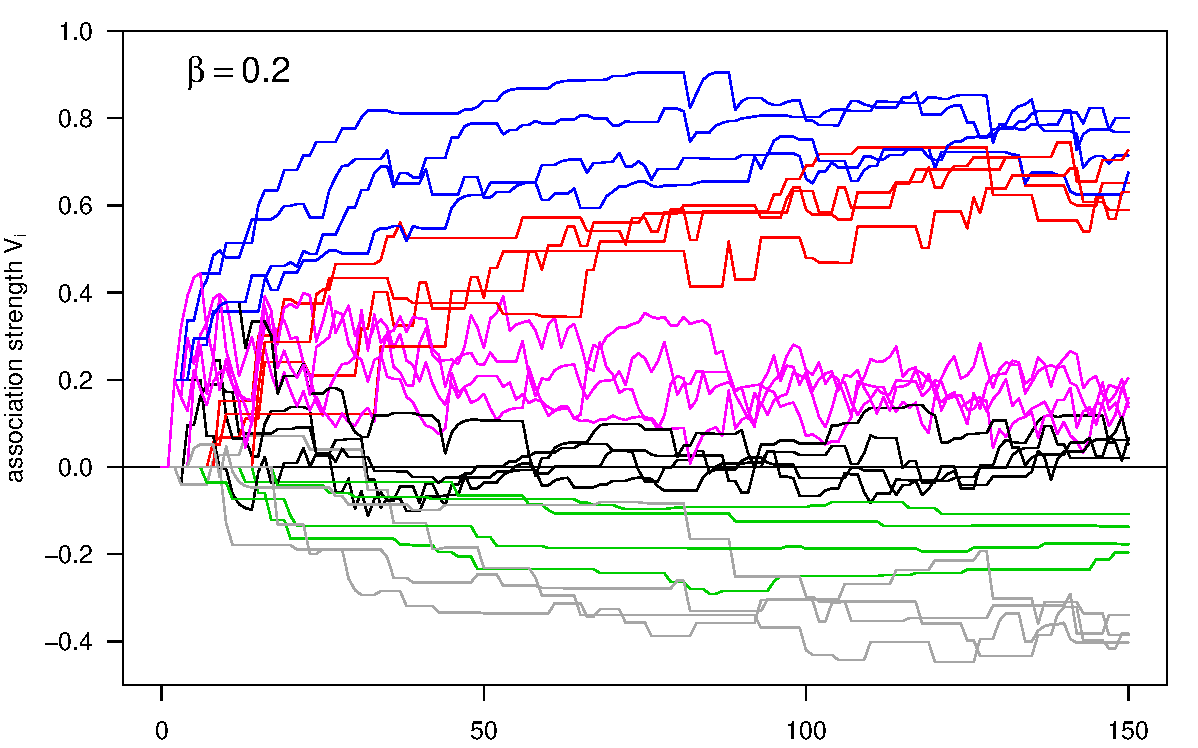
\includegraphics[width=10cm]{img/german_plural_exp_rw_step_4}}%
  \only<beamer:5| handout:0>{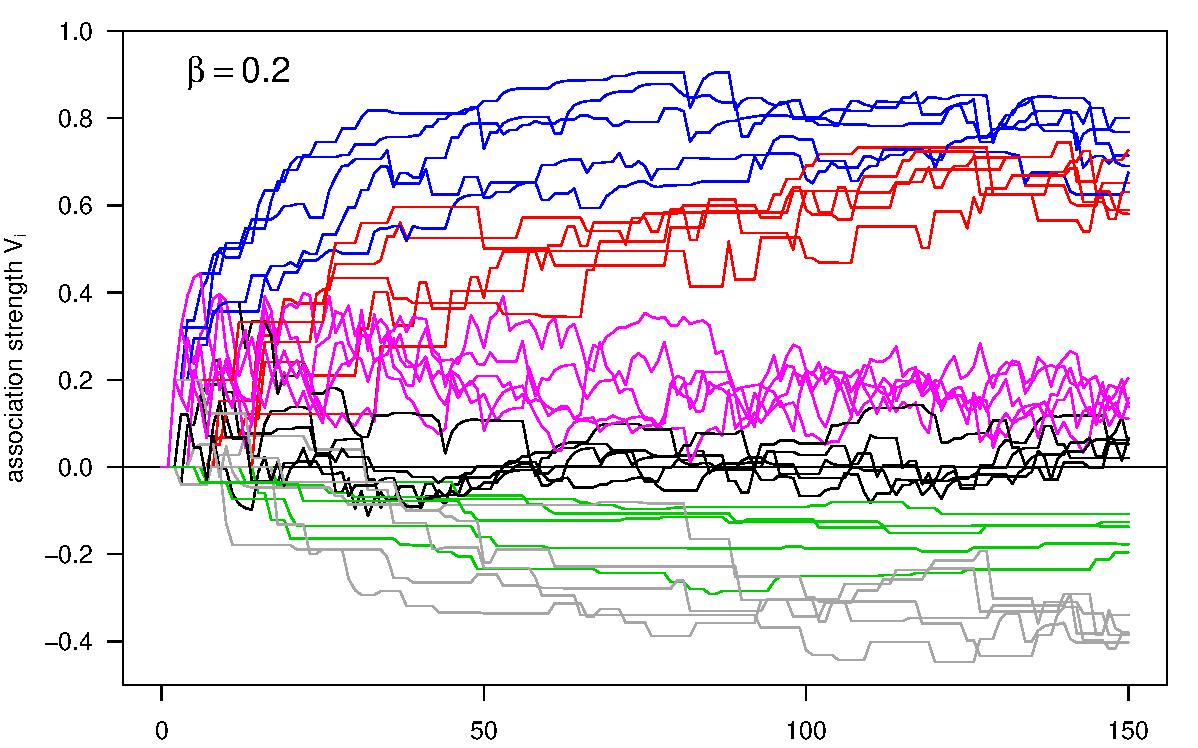
\includegraphics[width=10cm]{img/german_plural_exp_rw_step_5}}%
  \only<beamer:6| handout:1>{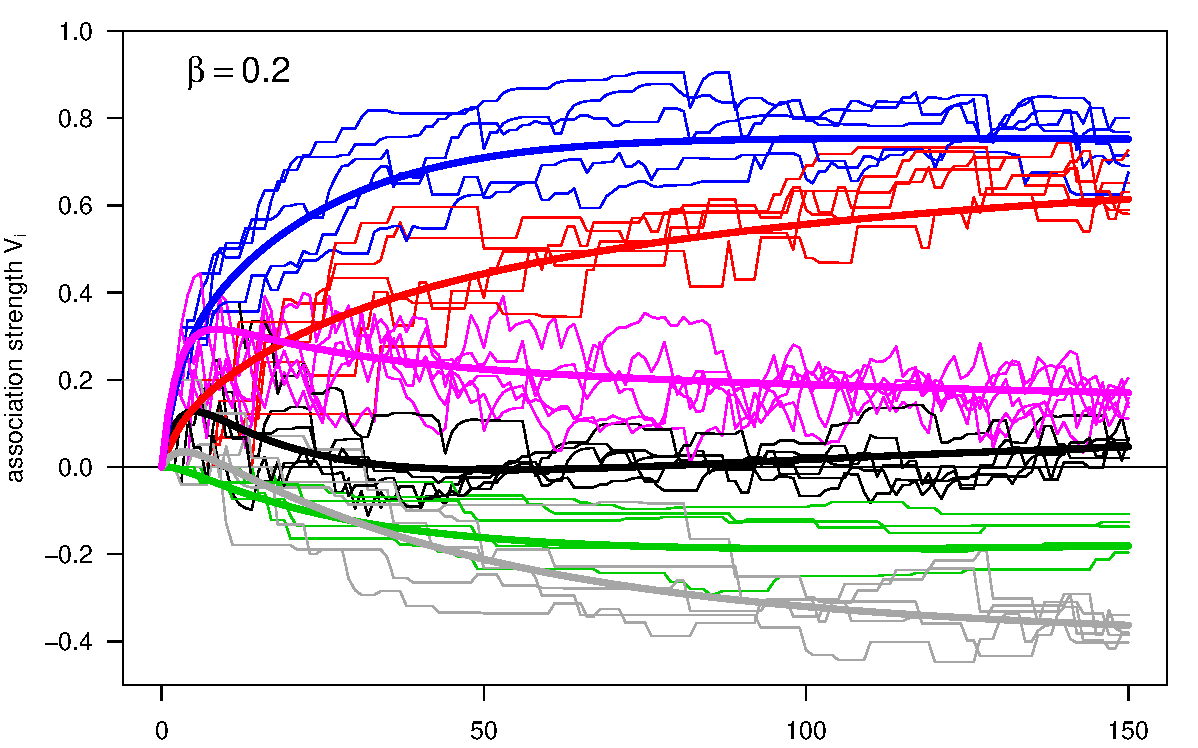
\includegraphics[width=10cm]{img/german_plural_exp_rw_final}}%
\end{frame}

\begin{frame}
  \frametitle{The Danks equilibrium}
  %% \framesubtitle{}

  \begin{itemize}
  \item If $\bigExp{V_i\psupt}$ converges, the asymptote $V_i^* = \lim_{t\to \infty} \bigExp{V_i\psupt}$ must satisfy the \primary{Danks equilibrium} conditions $\bigExp{\Delta V_i^*} = 0$, i.e.
    \[
    \p{C_i, O} - \textstyle\sum_{j=1}^n \p{C_i, C_j} V_j^* = 0 \quad \forall i
    \]
    \citep[p.~113]{Danks:03}
    \begin{itemize}
    \item[]
    \end{itemize}
  \item Now there is a clear interpretation of the Danks equilibrium as the stable average associations reached by a community of stochastic learners with input from the same population
    \begin{itemize}
    \item[\hand] allows us to compute the ``adult'' state of NDL without carrying out a simulation of the learning process
    \end{itemize}
  \end{itemize}
\end{frame}

\begin{frame}[c]
  \frametitle{The Danks equilibrium}
  %% \framesubtitle{}

  \centering
  \only<beamer:1| handout:0>{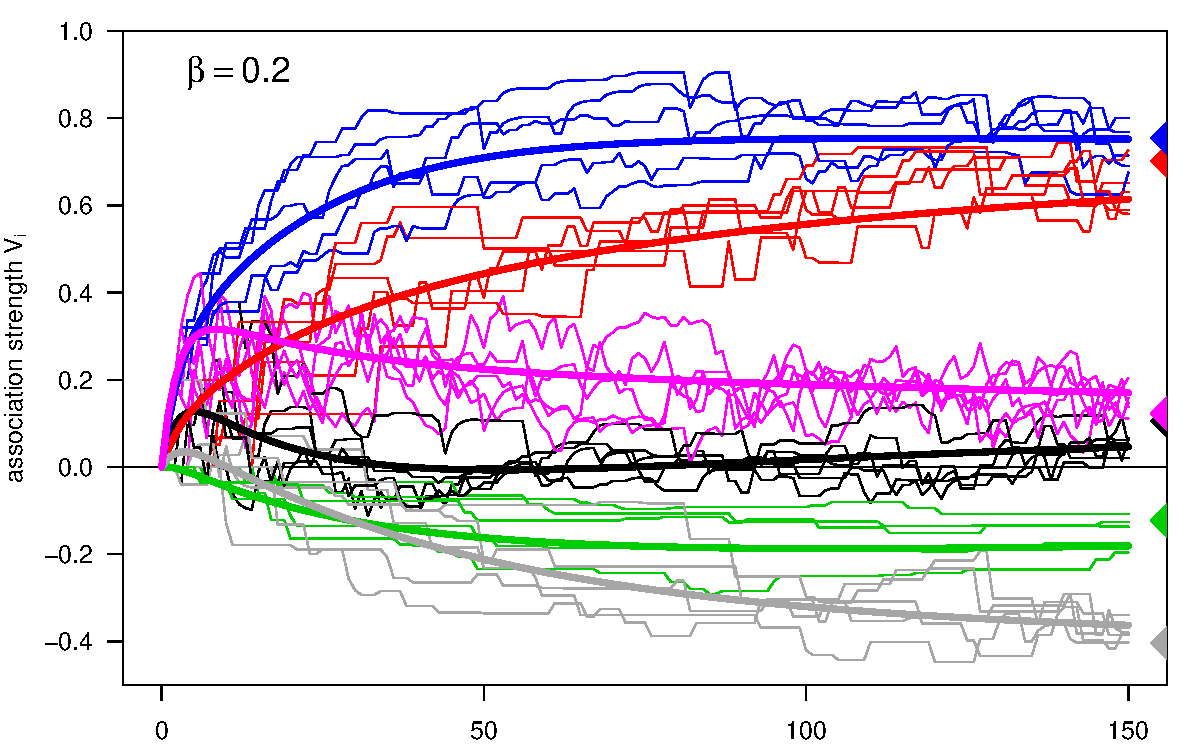
\includegraphics[width=11cm]{img/german_plural_exp_rw_danks}}%
  \only<beamer:2| handout:1>{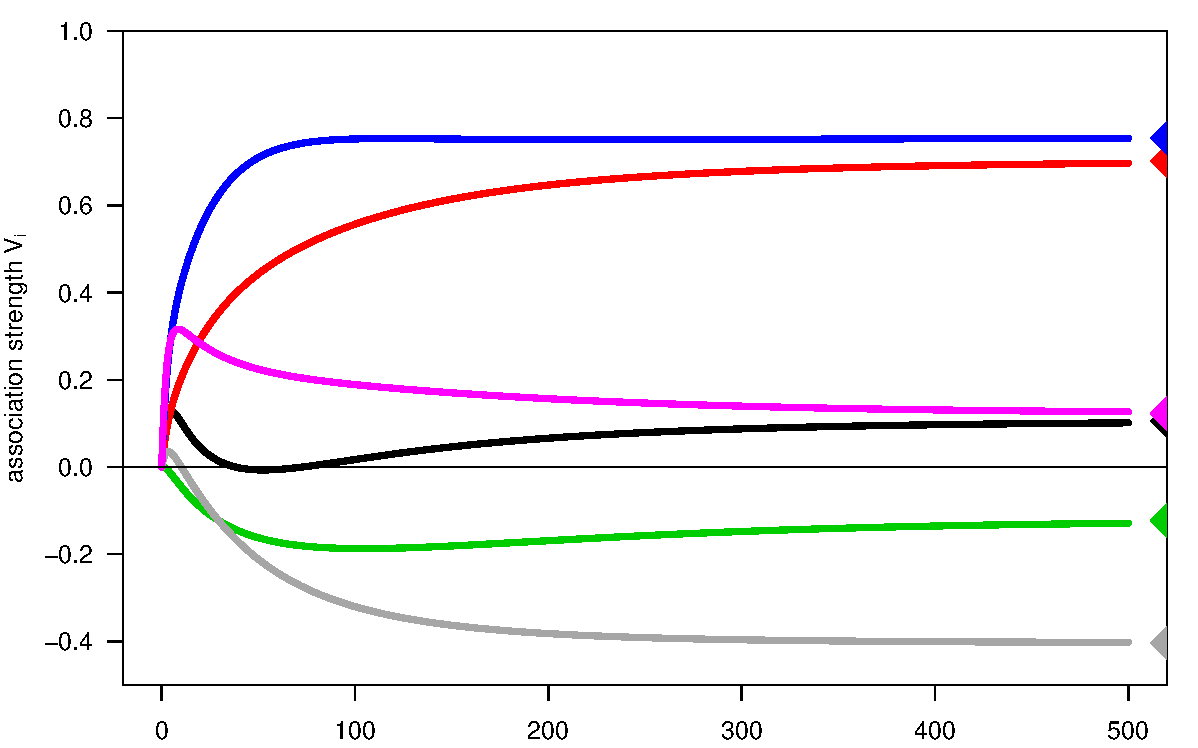
\includegraphics[width=11cm]{img/german_plural_exp_rw_danks_500}}%
\end{frame}

\begin{frame}
  \frametitle{Matrix notation}
  %% \framesubtitle{}
  
  \ungap[2]
  \begin{align*}
    \vX &=
    \begin{bmatrix}
      c_1\psup{1} & \cdots & c_n\psup{1} \\
      c_1\psup{2} & \cdots & c_n\psup{2} \\
      \vdots      &        & \vdots      \\
      c_1\psup{m} & \cdots & c_n\psup{m} 
    \end{bmatrix}
    &
    \vz &=
    \begin{bmatrix}
      o\psup{1} \\
      o\psup{2} \\
      \vdots \\
      o\psup{m}
    \end{bmatrix}
    &
    \vw &=
    \begin{bmatrix}
      V\psup{1} \\
      \vdots \\
      V\psup{n}
    \end{bmatrix}
  \end{align*}
  
  \begin{align*}
    \only<beamer:2-3| handout:0>{
    \small\begin{bmatrix} 
      f(C_1, O) \\ 
      \vdots \\
      f(C_n, O) 
    \end{bmatrix}
    &= \vX^T \vz
    &
    \visible<3->{
    \small\begin{bmatrix} 
      f(C_1, C_1) & \cdots & f(C_1, C_n) \\ 
      \vdots      &       & \vdots \\
      f(C_n, C_1) & \cdots & f(C_n, C_n)
    \end{bmatrix}
    &= \vX^T \vX
    }}%
    \only<beamer:4-| handout:1>{
    \small\begin{bmatrix} 
      \p{C_1, O} \\ 
      \vdots \\
      \p{C_n, O}
    \end{bmatrix}
    &= \tfrac{1}{m} \vX^T \vz
    &
    \small\begin{bmatrix} 
      \p{C_1, C_1} & \cdots & \p{C_1, C_n} \\ 
      \vdots      &       & \vdots \\
      \p{C_n, C_1} & \cdots & \p{C_n, C_n}
    \end{bmatrix}
    &= \tfrac{1}{m} \vX^T \vX
    }
  \end{align*}
  
  \gap[1]
  \[
  \visible<5->{\text{\primary{Danks equilibrium:}}} \quad
  \only<beamer:5| handout:0>{\tfrac{1}{m} \vX^T \vz - \tfrac{1}{m} \vX^T \vX \vw^* = \vnull}%
  \only<beamer:6-| handout:1>{\vX^T \vz = \vX^T \vX \vw^*}%
  \]
\end{frame}

\begin{frame}
  \frametitle{Matrix notation: German noun plurals}
  %% \framesubtitle{}
  
  \ungap[2]
  \begin{align*}
    \vX &=
    \footnotesize\begin{bmatrix}
      1 & 0 & 0 & 1 & 0 & 1 \\ 
      1 & 0 & 0 & 0 & 0 & 1 \\ 
      0 & 0 & 0 & 0 & 0 & 1 \\ 
      0 & 0 & 0 & 1 & 0 & 1 \\ 
      0 & 1 & 0 & 0 & 0 & 1 \\ 
      1 & 0 & 0 & 0 & 1 & 1 \\ 
      0 & 1 & 0 & 1 & 1 & 1 \\ 
      0 & 0 & 1 & 0 & 0 & 1 \\      
      1 & 0 & 0 & 1 & 0 & 1 \\ 
      1 & 0 & 0 & 1 & 0 & 1
    \end{bmatrix}
    &
    \vz &=
    \footnotesize\begin{bmatrix}
      1  \\
      0  \\
      0  \\
      1  \\
      1  \\
      0  \\
      1  \\
      0  \\
      1  \\
      1 
    \end{bmatrix}
    &
    \vw &=
    \begin{bmatrix}
      V\psup{1} \\
      \vdots \\
      V\psup{n}
    \end{bmatrix}
  \end{align*}
  
  \begin{align*}
    \only<beamer:1-3| handout:0>{
    \visible<2->{
    \small\begin{bmatrix} 
      3 \\ 
      2 \\
      0 \\
      5 \\
      1 \\
      6
    \end{bmatrix}
    &= \vX^T \vz}
    &
    \visible<3->{
    \small\begin{bmatrix} 
      5 & 0 & 0 & 3 & 1 &  5 \\ 
      0 & 2 & 0 & 1 & 1 &  2 \\ 
      0 & 0 & 1 & 0 & 0 &  1 \\ 
      3 & 1 & 0 & 5 & 1 &  5 \\ 
      1 & 1 & 0 & 1 & 2 &  2 \\ 
      5 & 2 & 1 & 5 & 2 & 10 
    \end{bmatrix}
    &= \vX^T \vX}
    }%
    \only<beamer:4-| handout:1>{
    \small\begin{bmatrix} 
      .3 \\ 
      .2 \\
      .0 \\
      .5 \\
      .1 \\
      .6
    \end{bmatrix}
    &= \tfrac{1}{m} \vX^T \vz
    &
    \small\begin{bmatrix} 
      .5 & .0 & .0 & .3 & .1 &  .5 \\ 
      .0 & .2 & .0 & .1 & .1 &  .2 \\ 
      .0 & .0 & .1 & .0 & .0 &  .1 \\ 
      .3 & .1 & .0 & .5 & .1 &  .5 \\ 
      .1 & .1 & .0 & .1 & .2 &  .2 \\ 
      .5 & .2 & .1 & .5 & .2 &  1 
    \end{bmatrix}
    &= \tfrac{1}{m} \vX^T \vX
    }
  \end{align*}
\end{frame}

%%% Local Variables: 
%%% mode: latex
%%% TeX-master: "../qitl6_evert_arppe"
%%% End: 


\subsection{NDL vs.\ the Perceptron vs.\  regression}

\tikzset{input/.style={basic,circle}}
\tikzset{weights/.style={basic,rectangle}}
\tikzset{functions/.style={basic,circle,fill=faugold!10}}
\tikzset{basic/.style={draw,fill=faublue!10,text width=1em,text badly centered}}
%% \tikzset{flow/.style={draw,-{>[scale=1.2]}}} % nicer, but only works with PGF 3.0
\tikzset{flow/.style={draw,->}} % nicer, but only works with PGF 3.0

\begin{frame}
  \frametitle{The single-layer perceptron (SLP)}
  %% \framesubtitle{}

  \begin{columns}[c]
    \begin{column}{6cm}
      SLP \citep{Rosenblatt:58} is most basic feed-forward \primary{neural network}
      \begin{itemize}
      \item<1-> numeric inputs $x_1, \ldots, x_n$
      \item<1-> output activation $h(y)$ based on weighted sum of inputs
        \[
        y = \textstyle\sum_{j=1}^n w_j x_j
        \]
      \item<2-> $h$ = Heaviside step function in traditional SLP
      \item<3-> even simpler model: $h(y) = y$
      \item<4-> cost wrt.\ target output $z$:
        \[
        E(\vw, \vx, z) = \left( z - \textstyle\sum_{j=1}^n w_j x_j \right)^2
        \]
      \end{itemize}
    \end{column}
    \begin{column}{5cm}
      \begin{tikzpicture}
        \node[functions] (center) {};
        \node[below=0.5em of center,font=\scriptsize,text width=3.4em] {activation function $h$};
        \draw (0em,0.75em) -- (0em,-0.75em);
        \draw (0.75em,0em) -- (-0.75em,0em);
        \only<beamer:1-2| handout:0>{
          \draw[very thick, color=primary] (0.7em,0.5em) -- (0,0.5em) -- (0,-0.5em) -- (-0.7em,-0.5em);
        }
%%        \draw[very thick, color=primary] (0.7em,0.5em) .. controls (-0.2em,0.5em) and (0.2em,-0.5em) .. (-0.7em,-0.5em);
        \only<beamer:3-| handout:1>{
          \draw[very thick, color=primary] (0.6em,0.6em) -- (-0.6em,-0.6em);
        }
        \node[right of=center] (right) {};
        \path[flow] (center) -- (right);
        \node[functions,left=1.5em of center] (left) {$\sum$};
        \path[flow] (left) -- (center);
        \node[weights,above left=0.5em and 2em of left] (2) {$w_2$} -- (2) node[input,left=1em of 2] (l2) {$x_2$};
        \path[flow] (l2) -- (2);
        \path[flow] (2) -- (left);
        \node[below of=2] (dots) {$\vdots$} -- (dots) node[below of=l2] (ldots) {$\vdots$};
        \node[weights,below of=dots] (n) {$w_n$} -- (n) node[input,left=1em of n] (ln) {$x_n$};
        \path[flow] (ln) -- (n);
        \path[flow] (n) -- (left);
        \node[weights,above of=2] (1) {$w_1$} -- (1) node[input,left=1em of 1] (l1) {$x_1$};
        \path[flow] (l1) -- (1);
        \path[flow] (1) -- (left);
        \node[below=1.5em of ln.center,font=\scriptsize] {inputs};
        \node[below=1.5em of n.center,font=\scriptsize] {weights};
      \end{tikzpicture}
    \end{column}
  \end{columns}  
\end{frame}

\begin{frame}
  \frametitle{SLP training: the delta rule}
  %% \framesubtitle{}
  \begin{itemize}
  \item SLP weights are learned by \primary{gradient descent} training:\\
    for a single training item $(\vx, z)$ and learning rate $\delta > 0$
    \begin{align*}
      \Delta w_i &= -\delta \frac{\partial E(\vw, \vx, z)}{\partial w_i} \\
      \only<beamer:1-2| handout:0>{\visible<2->{&= -\delta \frac{\partial}{\partial w_i} \left( z - \sum_{j=1}^n w_j x_j \right)^2 \\}}
      \only<beamer:3-4| handout:0>{&= -2\delta \left( z - \sum_{j=1}^n w_j x_j \right) (-x_i) \\}
      \only<beamer:5-| handout:1>{&= 2\delta x_i \left( z - \sum_{j=1}^n x_ j w_j \right) \\}
      \visible<4->{&= \secondary{\beta c_i \bigl( o - \textstyle\sum_{j=1}^n c_j V_j \bigr)}}
    \end{align*}
  \item<6-> Perfect \primary{correspondence to W-H rule} with
    \[
    V_i = w_i \qquad c_i = x_i \qquad o = z \qquad \beta = 2\delta
    \]
  \end{itemize}
\end{frame}

\begin{frame}
  \frametitle{Batch training}
  %% \framesubtitle{}

  \begin{itemize}
  \item Neural networks often use \primary{batch training}, where all training data are considered at once instead of one item at a time
  \item The corresponding batch training cost is
    \begin{align*}
    E(\vw) &= \frac{1}{m} \sum_{k=1}^m E(\vw, \vx[k], z\psup{k}) \\
    \visible<3->{ &= \frac{1}{m} \sum_{k=1}^m \left( z\psup{k} - \textstyle\sum_{j=1}^n w_j x_j\psup{k} \right)^2 }
    \end{align*}
  \item<2-> Similar to stochastic NDL, batch training computes the expected weights $\bigExp{\vw\psupt}$ for an SLP with stochastic input
  \item<3-> Minimization of $E(\vw)$ = linear \primary{least-squares regression}
  \end{itemize}
\end{frame}

\begin{frame}
  \frametitle{Linear least-squares regression}
  %% \framesubtitle{}
  
  \begin{itemize}
  \item Matrix formulation of the linear least-squares problem:
    \begin{align*}
      E(\vw) &= \frac{1}{m} \sum_{k=1}^m \left( z\psup{k} - \textstyle\sum_{j=1}^n w_j x_j\psup{k} \right)^2 \\
      \visible<2->{ &= \frac{1}{m} \bigl( \vz - \vX \vw \bigr)^T \bigl( \vz - \vX \vw \bigr) }
    \end{align*}
  \item<3-> Minimum of $E(\vw)$, the $L_2$ solution, must satisfy $\nabla E(\vw^*) = \vnull$, which leads to the \primary{normal equations}
    \[
    \vX^T \vz = \vX^T \vX \vw^*
    \]
  \item<4-> Normal equations = Danks equilibrium conditions
  \item<5-> Regression theory shows that batch training / stochastic NLP converges to the unique$^{\primary{*}}$ solution of the $L_2$ problem
  \end{itemize}
\end{frame}

\begin{frame}[c]
  \frametitle{What have we learned?}
  %% \framesubtitle{}

  \begin{center}\Large
    \setlength{\fboxrule}{2pt}
    \fcolorbox{secondary}{faugold!10!white}{
      \begin{tabular}{c c c c c}
        stochastic &=& batch &=& $L_2$ regression \\[1ex]
        NDL &=& SLP
      \end{tabular}
    }
  \end{center}
  \begin{itemize}
  \item[\hand] These equivalences also hold for the general R-W equations with arbitrary values of $\alpha_i$, $\beta_1$, $\beta_2$ and $\lambda$ (see paper)
  \end{itemize}
  
\end{frame}

%%% Local Variables: 
%%% mode: latex
%%% TeX-master: "../qitl6_evert_arppe"
%%% End: 


\subsection{The Danks equlibrium as least-squares regression}

\begin{frame}
  \frametitle{}
  %% \framesubtitle{}
\end{frame}

%%% Local Variables: 
%%% mode: latex
%%% TeX-master: "../qitl6_evert_arppe"
%%% End: 


%%%%%%%%%%%%%%%%%%%%%%%%%%%%%%%%%%%%%%%%%%%%%%%%%%%%%%%%%%%%%%%%%%%%%%
%% 3 Experiments

% \section{}

% \begin{frame}
  \frametitle{}
  %% \framesubtitle{}
\end{frame}

%%% Local Variables: 
%%% mode: latex
%%% TeX-master: "../workspace"
%%% End: 


%%%%%%%%%%%%%%%%%%%%%%%%%%%%%%%%%%%%%%%%%%%%%%%%%%%%%%%%%%%%%%%%%%%%%%
%% 4 Conclusion

\AtBeginSection[] % because we don't have a subsection here
{
  \begin{frame}
    \frametitle{Outline}
    \tableofcontents[current]
  \end{frame}
}

\section{Conclusion}

\begin{frame}
  \frametitle{Summary \& next steps}
  %% \framesubtitle{}
  \begin{center}
    \setlength{\fboxrule}{1pt}
    \fcolorbox{secondary}{faugold!10!white}{
      \begin{tabular}{c c c c c}
        stochastic &=& batch &=& $L_2$ regression \\[1ex]
        NDL &=& SLP
      \end{tabular}
    }
  \end{center}
  
  \begin{itemize}
  \item<2-> How many training steps are needed for a stochastic NDL learner to
    converge to the Danks equilibrium?
  \item<3-> Are there cases of non-convergence? If yes, why?
  \item<4-> Does NDL accuracy always improve with more cues and more training data?
      If not, why?
  \item<5-> How does logistic regression behave as incremental learner?
  \item<6-> Which sequences / patterns in the input data lead to significantly
    different behaviour from stochastic learner?
  \end{itemize}

\end{frame}

%%% Local Variables: 
%%% mode: latex
%%% TeX-master: "../qitl6_evert_arppe"
%%% End: 


\begin{frame}
  \frametitle{Acknowledgements}
  %% \framesubtitle{}

  \ungap[1]
  \begin{columns}[T]
    \begin{column}{55mm}
      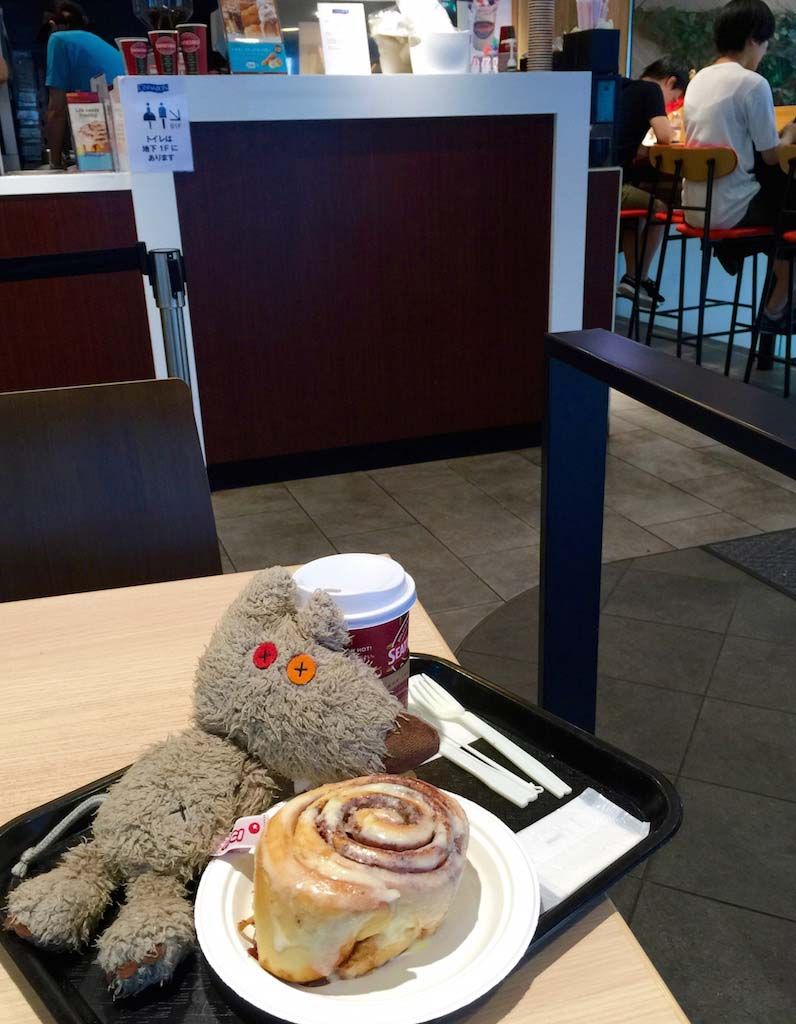
\includegraphics[width=52mm]{img/ratti_cinnamon_rolls}
      
      \scriptsize
      Follow me on Twitter: \secondary{@RattiTheRat}
    \end{column}
    \begin{column}{50mm}
      The mathematical analysis was fuelled by large amounts of coffee and cinnamon rolls at Cinnabon, Harajuku, Tokyo

    \end{column}
  \end{columns}
\end{frame}

%%% Local Variables: 
%%% mode: latex
%%% TeX-master: "../qitl6_evert_arppe"
%%% End: 


%%%%%%%%%%%%%%%%%%%%%%%%%%%%%%%%%%%%%%%%%%%%%%%%%%%%%%%%%%%%%%%%%%%%%%
%% References (if any)

\frame[allowframebreaks]{
  \frametitle{References}
  \bibliographystyle{natbib-stefan}
  \begin{scriptsize}
    \bibliography{references}
  \end{scriptsize}
}

\end{document}
